\documentclass[titlepage,11pt]{article}
\usepackage{comment}
\usepackage{enumitem}
\usepackage{listings}
\usepackage{amsmath}
\usepackage{graphicx}
\usepackage[font=small,labelfont=bf]{caption}
\usepackage[bahasa]{babel}
\usepackage{float}
\usepackage{verbatim}
\usepackage{graphicx,tabularx,multirow}
\usepackage{xcolor}
\usepackage[onehalfspacing]{setspace}
\usepackage[
	allcolors=visigrey,
	colorlinks=true,
]{hyperref}
\usepackage[a4paper,left=2cm,right=2cm]{geometry}
% Pengaturan kutipan artikel
\usepackage[style=ieee, backend=biber]{biblatex}
%Code listing style pak akok
\definecolor{codegreen}{rgb}{0,0.6,0}
\definecolor{codegray}{rgb}{0.5,0.5,0.5}
\definecolor{codepurple}{rgb}{0.58,0,0.82}
\definecolor{backcolour}{rgb}{0.95,0.95,0.92}

% Ubah sesuai modul
% \addbibresource{P1/pustaka/pustaka.bib}
\addbibresource{P2/pustaka/pustaka.bib}
% \addbibresource{P3/pustaka/pustaka.bib}
% \addbibresource{P4/pustaka/pustaka.bib}
% \addbibresource{P5/pustaka/pustaka.bib}

\lstdefinestyle{mystyle}{
	backgroundcolor=\color{backcolour}, commentstyle=\color{codegreen},
	keywordstyle=\color{magenta},
	numberstyle=\small\color{codegray},
	stringstyle=\color{codepurple},
	basicstyle=\ttfamily\footnotesize,
	breakatwhitespace=false,         
	breaklines=true,                 
	captionpos=t,                    
	keepspaces=true,                 
	numbers=left,                    
	numbersep=5pt,                  
	showspaces=false,                
	showstringspaces=false,
	showtabs=false,           
	frame = single,
	tabsize=2
}
\lstset{style=mystyle}

\definecolor{visigrey}{rgb}{.1,.15,.15}
\geometry{top=1cm,bottom=.5cm}
\savegeometry{titlepage}
\geometry{top=2cm,bottom=2cm}
\savegeometry{main}

\def\bspace{\(\qquad\qquad\qquad\)}
\usepackage[T1]{fontenc}
\usepackage[utf8]{inputenc}
\usepackage{tgheros}
\renewcommand*\familydefault{\sfdefault}

\setcounter{tocdepth}{6}

\def\autor{Laboratorium }
\def\lab{Multimedia dan Internet of Things}
\def\departemen{Departemen Teknik Komputer}
\def\institut{Institut Teknologi Sepuluh Nopember}
\def\praktikum{Praktikum \\ Jaringan Komputer}
% Ubah Judul sesuai dengan modul
% \def\judul{Wireless}
% \def\judul{Routing Static dan Routing Dinamis (Mikrotik)}
% \def\judul{Mengelola dan Membagi Bandwith menggunakan Qos(Simple Queue)}
\def\judul{VPN(Virtual Private Network) PPTP Pada Mikrotik}
% \def\judul{Implemntasi dan Konfigurasi IP Version 6}
\def\tahun{2024}
\begin{document}
% Ubah Bahasa sesuai dengan keinginan
\selectlanguage{bahasa}
\input{Cover/Header.tex}
% Pilih Modul yang akan di build
% \section{Pendahuluan}
\subsection{Latar Belakang}
Pada Wireless Jaringan Komputer, terdapat setidaknya 3 jenis, yaitu Point-to-Point Protocol
(PPP), Point-to-multipoint dan Wireless Bridging.\\\\
Point-to-Point Protocol (PPP) adalah data link protokol yang umum digunakan dalam
membangun hubungan langsung antara dua node jaringan. Hal ini dapat menyediakan koneksi
otentikasi, transmisi enkripsi (menggunakan ECP, RFC 1968), dan kompresi. Jenis ini
biasanya digunakan untuk menghubungkan jaringan antar 2 gedung atau antar 2 BTS (Base
Transceiver Station).\\\\
Point-to-multipoint adalah pendekatan yang paling populer untuk komunikasi nirkabel yang
memiliki banyak node, tujuan akhir atau pengguna akhir. Jenis ini biasanya digunakan untuk
membuat wifi atau hotspot yang berasal dari 1 sumber disebar ke banyak client dalam suatu
jaringan.\\\\
Wireless Bridging digunakan untuk menghubungkan dua segmen LAN melalui tautan
nirkabel. Kedua segmen akan berada di subnet yang sama dan terlihat seperti dua switch
Ethernet yang dihubungkan oleh kabel ke semua komputer di subnet.\\\\
Untuk mengembangkan jaringan komputer berbasis wireless yang berkualitas dan mempunyai
ketersediaan tinggi, penggunaan 3 jenis ini perlu disesuaikan dengan kebutuhan dan kondisi
nya, sehingga kali ini saya akan membahasnya 1 persatu dari 3 jenis koneksi wireless
tersebut.

%\begin{itemize}[label=$\bullet$, itemsep=-1pt, leftmargin=*]
%	\item Cek Halo
%\end{itemize}

\subsection{Maksud dan Tujuan}
Mengetahui dan memahami 3 jenis koneksi pada Jaringan Wireless.

\subsection{Hasil yang diharapkan}
Dapat mengkonfigurasi koneksi Wireless Bridge, Point to Point dan Point to Multipoint
dengan tepat.

%===========================================================%
\section{Tugas Pendahuluan}
\begin{enumerate}
	\item Halo
\end{enumerate}

\begin{center}
	\colorbox{cyan!30}{\parbox{0.8\linewidth}{\textbf{Opsional:} Pelajari Git dan Github. Anda dapat memulai pembelajaran dari sumber berikut ini: \\ \href{https://github.com}{GitHub - https://github.com} \\ \href{https://git-scm.com/doc}{Git -https://git-scm.com/doc}}}
\end{center}

%===========================================================%
\section{Alat dan Bahan}
\begin{itemize}[label=$\bullet$, itemsep=-1pt, leftmargin=*]
	\item 2 atau lebih perangkat router mikrotik yang sudah support wireless.
	\item Aplikasi Winbox.
\end{itemize}

%===========================================================%
\section{Jangka Waktu Pelaksanaan}
Pemahaman dan konfigurasi 1 jam.

%===========================================================%
\section{Proses dan Tahapan Konfigurasi}

\subsection{Wireless Point to Point}
Untuk koneksi Point to Point seperti contohnya topologi seperti dibawah ini, biasanya
digunakan untuk menghubungkan 2 router atau 2 node jaringan, Hal ini dilakukan biasanya
untuk koneksi koneksi jarak jauh yang mengharapkan kecepatan tinggi misal untuk
menghubungkan jaringan antar gedung, menghubungkan BTS (Base Transceiver Station) to
BTS (Base Transceiver Station). Koneksi point to point ini akan lebih aman karena maksimal
node yang terhubung hanya 2. Untuk konfigurasinya seperti berikut ini.

\begin{center}
	\begin{enumerate}
		\item Buatlah skenario topologi seperti gambar dibawah ini, Router1 (Router Utama) menjadi mode Bridge dan Router 2 menjadi mode Station.
		\begin{figure}[H]
			\centering
			\includegraphics[width=0.7\linewidth]{P1/img/contoh.png}
			\caption{Gambar Contoh}
			\label{fig:gambarcontoh}
		\end{figure}
		\item Konfigurasi wireless mode Bridge pada Router1 seperti berikut ini.
		\begin{figure}[H]
			\centering
			\includegraphics[width=0.7\linewidth]{P1/img/contoh.png}
			\caption{Gambar Contoh}
			\label{fig:gambarcontoh}
		\end{figure}
		\item Untuk konfigurasi IP sesuaikan dengan kebutuhan kalian, saya contohkan seperti dibawah ini.
		\begin{figure}[H]
			\centering
			\includegraphics[width=0.7\linewidth]{P1/img/contoh.png}
			\caption{Gambar Contoh}
			\label{fig:gambarcontoh}
		\end{figure}
		\item Pada Router2 konfigurasi mode Station seperti dibawah ini, namun sebelumnya silahkan Scan dan connectkan dengan SSID yang telah diatur di Router1 yaitu PointToPointLur.
		\begin{figure}[H]
			\centering
			\includegraphics[width=0.7\linewidth]{P1/img/contoh.png}
			\caption{Gambar Contoh}
			\label{fig:gambarcontoh}
		\end{figure}
		\item Setelah itu setting IP yang satu subnet dengan Router1.
		\begin{figure}[H]
			\centering
			\includegraphics[width=0.7\linewidth]{P1/img/contoh.png}
			\caption{Gambar Contoh}
			\label{fig:gambarcontoh}
		\end{figure}
		\item Selanjutnya silahkan ping IP Router2 dari Router1 seperti berikut ini.
		\begin{figure}[H]
			\centering
			\includegraphics[width=0.7\linewidth]{P1/img/contoh.png}
			\caption{Gambar Contoh}
			\label{fig:gambarcontoh}
		\end{figure}
		\item Ping IP Router1 dari Router2 seperti berikut ini. Jika TTL maka konfigurasi PointToPoint berhasil.
		\begin{figure}[H]
			\centering
			\includegraphics[width=0.7\linewidth]{P1/img/contoh.png}
			\caption{Gambar Contoh}
			\label{fig:gambarcontoh}
		\end{figure}
		\item Tambahan saja, pada Router2 kalian dapat cek di registration Tx dan Rx yang didapat serta kekuatan sinyal seperti berikut.
		\begin{figure}[H]
			\centering
			\includegraphics[width=0.7\linewidth]{P1/img/contoh.png}
			\caption{Gambar Contoh}
			\label{fig:gambarcontoh}
		\end{figure}
	\end{enumerate}
\end{center}

\subsection{Wireless Point to Multipoint}
Koneksi ini yang paling banyak digunakan, karena kelebihannya yaitu dapat mengkoneksikan
multipoint atau banyak node dari satu point atau node sumber, penerapan pada koneksi ini
biasanya berupa hotspot. Untuk konfigurasinya seperti berikut.
Untuk gambar topologi sama dengan PointToPoint, hanya saja berbeda di konfigurasi dan
mode pada routernya.
\begin{center}
	\begin{enumerate}
		\item Buatlah mode AP Bridge di router yang dijadikan router utama seperti berikut.
		\item Kemudian setting IP pada wlan1 sesuai keinginan kalian, disini saya konfigurasi IP seperti berikut.
		\item Pada Router Station, pergi ke pengaturan wireless dan lakukan scan, kemudian connectkan dengan SSID yang telah di setting di Router utama yaitu PointToMultiPointLur.
		\item Settingannya seperti berikut.
		\item Lakukan juga konfigurasi IP pada wlan1 yang satu subnet dengan Router Utama.
		\item Setelah itu silahkan cek PING dari router AP Bridge ke station.
		\item PING dari router station ke AP Bridge. Jika TTL maka koneksi telah berhasil terhubung.
		\item Kalian juga bisa menghubungkan laptop kalian ke router1 atau router utama melalui koneksi wifi yang sudah dibuat, pastikan laptop kalian IP nya sudah di setting 1 network, dan lakukan PING dari laptop kalian ke IP Router1 atau router wifi.
	\end{enumerate}
\end{center}

\subsection{Wireless Bridge}
Untuk wireless bridge ini sangatlah sederhana, koneksi ini sangat jarang ditemui pada
implementasi realnya, konfigurasi ini menjadikan seolah-olah koneksi yang terhubung
menggunakan switch, keunggulan yang saya rasakan yaitu ringannya kinerja router yang
menggunakan koneksi ini. Untuk konfigurasinya seperti berikut.
Untuk gambar topologi sama dengan Point To Point, hanya saja berbeda di konfigurasi dan
mode pada routernya.
\begin{center}
	\begin{enumerate}
		\item Setting pada Router1 sebagai mode bridge dan SSID sebagai berikut.
		\item Konfigurasi IP pada interface wlan1 yang terhubung ke router dan ether2 yang terhubung ke Laptop seperti berikut.
		\item Tambahkan bridge pada router1 seperti berikut.
		\item Dan tambahkan Port pada bridge untuk wlan dan ether2, kemudia apply>ok.
		\item Pada Router2, lakukan konfigurasi dengan mode station pseoubridge seperti berikut, setelah itu scan dan konekan dengan SSID yang telah di setting di Router1.
		\item Setting IP pada interface wlan1 yang terhubung ke router dan ether2 yang terhubung ke laptop seperti berikut.
		\item Tambahan saja, untuk anda dapat gunakan access list untuk mengkontrol setiap perangkat yang terhubung dengan MAC.
		\item Lakukan konfigurasi IP pada laptop yg terhubung ke Router1 seperti berikut.
		\item Lakukan konfigurasi IP pada laptop yg terhubung ke Router2 seperti berikut.
		\item Setelah semua terkonfigurasi. Lakukan PING dari kedua router seperti berikut, jika saling TTL maka kedua router telah terhubung.
		\item Lakukan juga PING antar laptop seperti berikut. jika reply maka konfigurasi Wireless Bridge berhasil.
	\end{enumerate}
\end{center}

%===========================================================%
\section{Hasil yang didapat}
Memahami dan mengkonfigurasi koneksi Point to Point, Point to Multipoint dan Wireless
Bridging dengan tepat.

%===========================================================%
\section{Temuan Permasalahan}
Firewall hidup pada Laptop dapat mempengaruhi koneksi wireless tidak terhubung, kalian
bisa menonaktifkan firewall di laptop kalian, tetapi hal ini tidak terjadi di semua perangkat.

%===========================================================%
\section{Kesimpulan}
Dengan memahami dan mengkonfigurasi 3 jenis koneksi pada wireless, kita dapat
mengimplementasikan koneksi wireless dengan tepat sesuai kebutuhan dan kondisi tertentu.

\cite{Newton1687}.
% \section{Pendahuluan}
\subsection{Latar Belakang}
Pada modul ini, kita akan membahas konfigurasi routing static dan routing dinamis pada perangkat
MikroTik. Routing merupakan proses pengiriman data antara dua atau lebih jaringan yang berbeda.
Dalam modul ini, kita akan membahas konsep dasar routing, macam-macam routing statis dan
dinamis, serta langkah-langkah untuk mengkonfigurasi kedua jenis routing ini pada perangkat
MikroTik.\\\\
Sebelum memulai pembahasan routing, penting untuk memahami konsep dasar jaringan dan
subnetting. Jaringan terdiri dari sejumlah perangkat yang terhubung satu sama lain, seperti komputer,
printer, dan perangkat jaringan lainnya. Setiap perangkat dalam jaringan memiliki alamat IP yang
unik.\\\\
Subnetting adalah proses pembagian jaringan menjadi subnet yang lebih kecil. Dengan subnetting, kita
dapat mengoptimalkan penggunaan alamat IP dan membagi jaringan menjadi beberapa segmen yang
terpisah.\\\\
Dalam routing, terdapat yang namanya protokol routing. Protokol routing adalah aturan yang
digunakan oleh perangkat jaringan untuk memilih jalur terbaik bagi pengiriman data antara jaringan
yang berbeda. Ada dua jenis protokol routing utama: \textbf{routing static dan routing dinamis.}\\\\

\subsection{Maksud dan Tujuan}
Mengetahui dan memahami konfigurasi routing static dan routing dinamis pada Mikrotik.

\subsection{Hasil yang diharapkan}
Dapat mengkonfigurasi konfigurasi routing static dan routing dinamis pada Mikrotik dengan
tepat.

%===========================================================%
\section{Tugas Pendahuluan}
\begin{enumerate}
	\item Halo
\end{enumerate}

\begin{center}
	\colorbox{cyan!30}{\parbox{0.8\linewidth}{\textbf{Opsional:} Pelajari Git dan Github. Anda dapat memulai pembelajaran dari sumber berikut ini: \\ \href{https://github.com}{GitHub - https://github.com} \\ \href{https://git-scm.com/doc}{Git -https://git-scm.com/doc}}}
\end{center}

%===========================================================%
\section{Alat dan Bahan}
\begin{itemize}[label=$\bullet$, itemsep=-1pt, leftmargin=*]
	\item 2 perangkat router mikrotik.
	\item Aplikasi Winbox.
	\item 3 kabel LAN
\end{itemize}

%===========================================================%
\section{Jangka Waktu Pelaksanaan}
Pemahaman dan konfigurasi 1 jam.

%===========================================================%
\section{Penjelasan dan Tahapan Konfigurasi}

\subsection{Routing Statis}
Pada routing statis, terdapat setidaknya 2 jenis, yaitu
\begin{enumerate}
	\item Default Route : digunakan ketika tidak ada rute spesifik yang cocok untuk tujuan pengiriman data. Jika tidak ada rute yang cocok, paket data akan dikirim melalui default route. Pada MikroTik, default route dinyatakan sebagai 0.0.0.0/0.
	\item Static Route : adalah jenis routing di mana administrator jaringan secara manual mengonfigurasi tabel routing pada setiap perangkat jaringan. Dalam routing static, rute yang ditentukan secara manual digunakan untuk mengarahkan paket data ke tujuan yang ditentukan.
\end{enumerate}
Pada kesempatan kali ini, kita akan membuat routing jenis static route, Tahap awal kalian
perlu membuat topologi dan konfigurasi IP Address nya sebagai berikut :\\
===Gambar===\\Berikut penjelasan dan tahapan konfigurasinya.
\begin{center}
	\textbf{Konfigurasi Router1}
\end{center}

	\begin{enumerate}
		\item Pertama kita login ke mikrotik dengan winbox
		\item Setelah masuk ke winbox, kita masuk ke ip --> address lalu kita atur ipnya router 1 eth3, ip address 10.10.50.1/28, eth2, ip address 192.168.80.2/28
		\item Lalu kita masuk ke ip --> route --> klik add(+), lalu pada Dst.Address isikan 172.16.2.0/24 (ip network client yang ada pada router2) dan pada gateway isikan 10.10.50.2 (ip yang terhubung dari router2 ke router1), klik apply --> ok
		\item Jika sudah maka akan reachable eth3
		\item Sekarang kita konfigurasi pada DHCP servernya untuk client yang akan terhubung
		\item Kita coba untuk ping
	\end{enumerate}
\begin{center}
	\textbf{Konfigurasi Router2}
\end{center}
	\begin{enumerate}
		\item Seperti langkah diatas kita masuk dulu ke mikrotik dengan winbox
		\item Setelah masuk kita masuk ke ip --> address lalu kita atur ipnya router 2 eth3, ip address 10.10.50.2/28 eth2, ip address 192.168.80.2/28
		\item Lalu kita masuk ke ip --> route --> klik add(+), lalu pada Dst.Address isikan 192.168.80.0/28 (ip network client yang ada pada router1) dan pada gateway isikan 10.10.50.1 (ip yang terhubung dari router1 ke router2), klik apply --> ok
		\item Jika sudah maka akan reachable eth3
		\item Sekarang kita konfigurasi pada DHCP servernya untuk client yang akan terhubung
		\item Kita coba ping ke router1
		\item Tahap terakhir atau penugasan, setting IP Address pada PC client router1 dan router2, kemudian PING IP dari PC router2 ke PC Router2, pastikan berhasil dan lampirkan dalam laporan.
	\end{enumerate}

\subsection{Routing Dinamis}
Pada routing dinamis, terdapat setidaknya 3 jenis, yaitu
\begin{enumerate}
	\item Routing Information Protocol (RIP) RIP adalah salah satu protokol routing dinamis yang menggunakan metrik hop count (jumlah hop) untuk menentukan jalur terbaik. Metrik hop count mengukur jarak antara router pengirim dengan tujuan dalam jumlah hop (melalui berapa banyak router).
	\item Open Shortest Path First (OSPF) OSPF adalah protokol routing dinamis yang menggunakan algoritma Dijkstra untuk menentukan jalur terpendek. OSPF mengumpulkan informasi topologi dari semua router dalam jaringan dan menghitung jalur terbaik berdasarkan bobot (cost) setiap link.
	\item Border Gateway Protocol (BGP) BGP adalah protokol routing eksternal yang digunakan di Internet. BGP memungkinkan router di AS (Autonomous System) yang berbeda untuk berkomunikasi dan menukar informasi routing.
\end{enumerate}
Pada kesempatan kali ini, kita akan membuat routing jenis static route, Tahap awal kalian perlu membuat topologi dan konfigurasi IP Address nya sebagai berikut :\\
===Gambar===\\Penjelasan dan tahapan konfigurasi sebagai berikut :

\begin{center}
	\textbf{Konfigurasi Router1}
\end{center}
\begin{enumerate}
	\item Pertama kita buka winbox, lalu buat IP Address klik \textbf{IP > Address.}
	\item Lalu kita membuat IP Address yang menghubungkan interface router 1 dan router 2, pada konfigurasi ini saya menggunakan interface ether2 sebagai penghubungnya. $\Rightarrow$ \textbf{Address : 172.160.8.1/24 > Interface :} (biarkan kosong) > \textbf{Interface : ether.}
	\item Langkah selanjutnya kita mengatur IP Address yang terhubung dengan laptop. $\Rightarrow$ \textbf{Address : 192.168.10.1/24 > Interface : ether3 > Apply > Ok.}
	\item Selanjutnya kita klik \textbf{Routing > RIP.}
	\item Klik tab \textbf{Interfaces > Add > Interface : ether2} (interface yang menghubungkan antar router) \textbf{> receive : v1 > send : v1 > Apply > Ok.}
	\item Langkah selanjutnya memasukan semua IP Network ether2 dan ether3. $\Rightarrow$ klik tab \textbf{Networks > Add > Address : 172.160.8.0/24 > Ok.}
	\item Klik \textbf{Network > Add > Address : 192.160.10.0/24 > Ok.}
	\item Selanjutnya kita klik tab Neighbours, disini kita memasukan alamat IP tujuan router lawan. Klik \textbf{Add > Address : 172.160.8.2 > Ok.}
	\item Setelah konfigurasi router 1 selesai, selanjutnya kita konfigurasi IP laptop. $\Rightarrow$ \textbf{Address : 192.168.10.2 > Netmask : 255.255.255.0 > Gateway : 192.168.10.1.}
\end{enumerate}

\begin{center}
	\textbf{Konfigurasi Router2}
\end{center}
\begin{enumerate}
	\item Pertama kita buka winbox, lalu buat IP Address klik \textbf{IP > Address.}
	\item Lalu kita membuat IP Address yang menghubungkan interface router 1 dan router 2, pada konfigurasi ini saya menggunakan interface ether2 sebagai penghubungnya $\Rightarrow$ \textbf{Address : 172.160.8.2/24 > Interface : ether2 > Apply > Ok.}
	\item Langkah selanjutnya kita mengatur IP Address yang terhubung dengan laptop. $\Rightarrow$ \textbf{Address : 192.168.20.2/24 > Interface : ether3 > Apply > Ok.}
	\item Selanjutnya kita klik \textbf{Routing > RIP.}
	\item Klik tab \textbf{Interfaces > Add > Interface : ether2} (interface yang menghubungkan antar router) \textbf{> receive : v1 > send : v1 > Apply > Ok.}
	\item Langkah selanjutnya memasukan semua IP Network ether2 dan ether3 $\Rightarrow$ klik tab \textbf{Networks > Add > Address : 172.160.8.0/24 > Ok.}
	\item $\Rightarrow$ \textbf{Klik Network > Add > Address : 192.160.20.0/24 > Ok.}
	\item Selanjutnya kita klik tab Neighbours, disini kita memasukan alamat IP tujuan router lawan. Klik \textbf{Add > Address : 172.160.8.1 > Ok.}
	\item Setelah konfigurasi router 1 selesai, selanjutnya kita konfigurasi IP laptop. $\Rightarrow$ \textbf{Address : 192.168.20.3 > Netmask : 255.255.255.0 > Gateway : 192.168.20.2.}
\end{enumerate}

\begin{center}
	\textbf{Pengujian Konfigurasi}
\end{center}
Untuk mengetes apakah konfigurasi telah berhasil atau belum dapat dilakukan dengan melakukan ping masing - masing IP Address laptop lawan.\\
==Gambar==\\==Gambar==\\
Apabila masing - masing Laptop mendapatkan jawaban selamat konfigurasi berhasil.

%===========================================================%
\section{Hasil yang didapat}
Memahami dan mengkonfigurasi routing dinamis RIP dengan tepat.

%===========================================================%
\section{Kesimpulan}
Dalam mengkonfigurasi routing RIP, diperlukan pemahaman dasar mengenai setting IP Address dan Subnetting, dan juga diperlukan ketelitian dan fokus agar berhasil

\cite{Newton1687}.


% \section{Tujuan}
\begin{itemize}[label=$\bullet$, itemsep=-1pt, leftmargin=*]
    \item Cek Halo
\end{itemize}

\section{Mengenal Jaringan}
Halo halo

\begin{figure}[H]
    \centering
    \includegraphics[width=0.7\linewidth]{P3/img/contoh.png}
    \caption{Gambar Contoh}
    \label{fig:gambarcontoh}
\end{figure}

\subsection{Tugas Pendahuluan}
\begin{enumerate}
    \item Halo
\end{enumerate}


\begin{center}
    \colorbox{cyan!30}{\parbox{0.8\linewidth}{\textbf{Opsional:} Pelajari Git dan Github. Anda dapat memulai pembelajaran dari sumber berikut ini: \\ \href{https://github.com}{GitHub - https://github.com} \\ \href{https://git-scm.com/doc}{Git -https://git-scm.com/doc}}}
\end{center}
\section{Pendahuluan}
\subsection{Latar Belakang}
VPN atau Jaringan Pribadi Virtual (Virtual Private Network) membuat koneksi jaringan privat di
antara beberapa perangkat melalui internet. VPN digunakan untuk mentransmisikan data secara aman
dan anonim melalui jaringan publik. VPN bekerja dengan cara menyembunyikan alamat IP pengguna
dan mengenkripsi data sehingga tidak dapat dibaca oleh siapa pun yang tidak berwenang untuk
menerimanya.\\\\
Salah satu service yang biasa digunakan untuk membangun sebuah jaringan VPN adalah Point to
Point Tunnel Protocol (PPTP). Sebuah koneksi PPTP terdiri dari Server dan Client.
Mikrotik RouterOS bisa difungsikan baik sebagai server maupun client atau bahkan diaktifkan
keduanya bersama dalam satu mesin yang sama. Feature ini sudah termasuk dalam package PPP
sehingga anda perlu cek di menu system package apakah paket tersebut sudah ada di router atau
belum. Fungsi PPTP Client juga sudah ada di hampir semua OS, sehingga kita bisa menggunakan
Laptop/PC sebagai PPTP Client.\\\\
Biasanya PPTP ini digunakan untuk jaringan yang sudah melewati multihop router (Routed Network).
Jika anda ingin menggunakan PPTP pastikan di Router anda tidak ada rule yang melakukan blocking
terhadap protocol TCP 1723 dan IP Protocol 47/GRE karena service PPTP menggunakan protocol
tersebut.

\subsection{Maksud dan Tujuan}
Mengetahui cara menggunakan dan mengkonfigurasi VPN PPTP pada router mikrotik.

\subsection{Hasil yang diharapkan}
Memahami penerapan dan penghubungan jaringan dengan menerapkan PPTP dengan VPN

%===========================================================%
\section{Tugas Pendahuluan}
\begin{center}
	\colorbox{cyan!30}{\parbox{0.8\linewidth}{
    \begin{enumerate}
        \item Apa itu PPTP dan bagaimana cara kerjanya?
        \item Apa kelebihan dan kekurangan dari penggunaan PPTP dibandingkan protokol VPN lainnya seperti L2TP atau OpenVPN?
    \end{enumerate}}}
\end{center}

%===========================================================%
\section{Alat dan Bahan}
\begin{itemize}[label=$\bullet$, itemsep=-1pt, leftmargin=*]
	\item 2 buah Cloud Core Router
	\item 3 Kabel UTP (LAN)
	\item 2 buah Laptop
	\item Software Winbox
\end{itemize}

%===========================================================%
\section{Jangka Waktu Pelaksanaan}
Pemahaman dan konfigurasi 1 jam.

%===========================================================%
\section{Penjelasan dan Tahapan Konfigurasi}

%======================PERCOBAAN 1==========================%
\begin{center}
    \textbf{Konfigurasi PC 1}
    \begin{enumerate}
        \item Buka aplikasi Winbox pada PC dan lakukan hubungkan ke Router. Pastikan Login terisi “admin”, Klik Neighbors > Klik Refresh > Pilih Router yang ingin disambungkan > Klik Connect.
        \begin{figure}[H]
			\centering
			\includegraphics[width=0.5\linewidth]{P4/img/pc1/Step 1.png}
			\caption{Step 1}
			\label{fig:Step 1(PC 1)}
		\end{figure}
        \item Jadikan Router menjadi DHCP Client agar bisa mendapat IP address dari Internet ITS. IP > Klik DHCP Client > Tambahkan DHCP Client > Pilih interface yang terhubung dengan Internet (ether2)> Klik Apply > Klik OK. Kita bisa memastikan koneksi ke internet dengan cara melakukan tes ping ke alamat IP 8.8.8.8
        \begin{figure}[H]
			\centering
			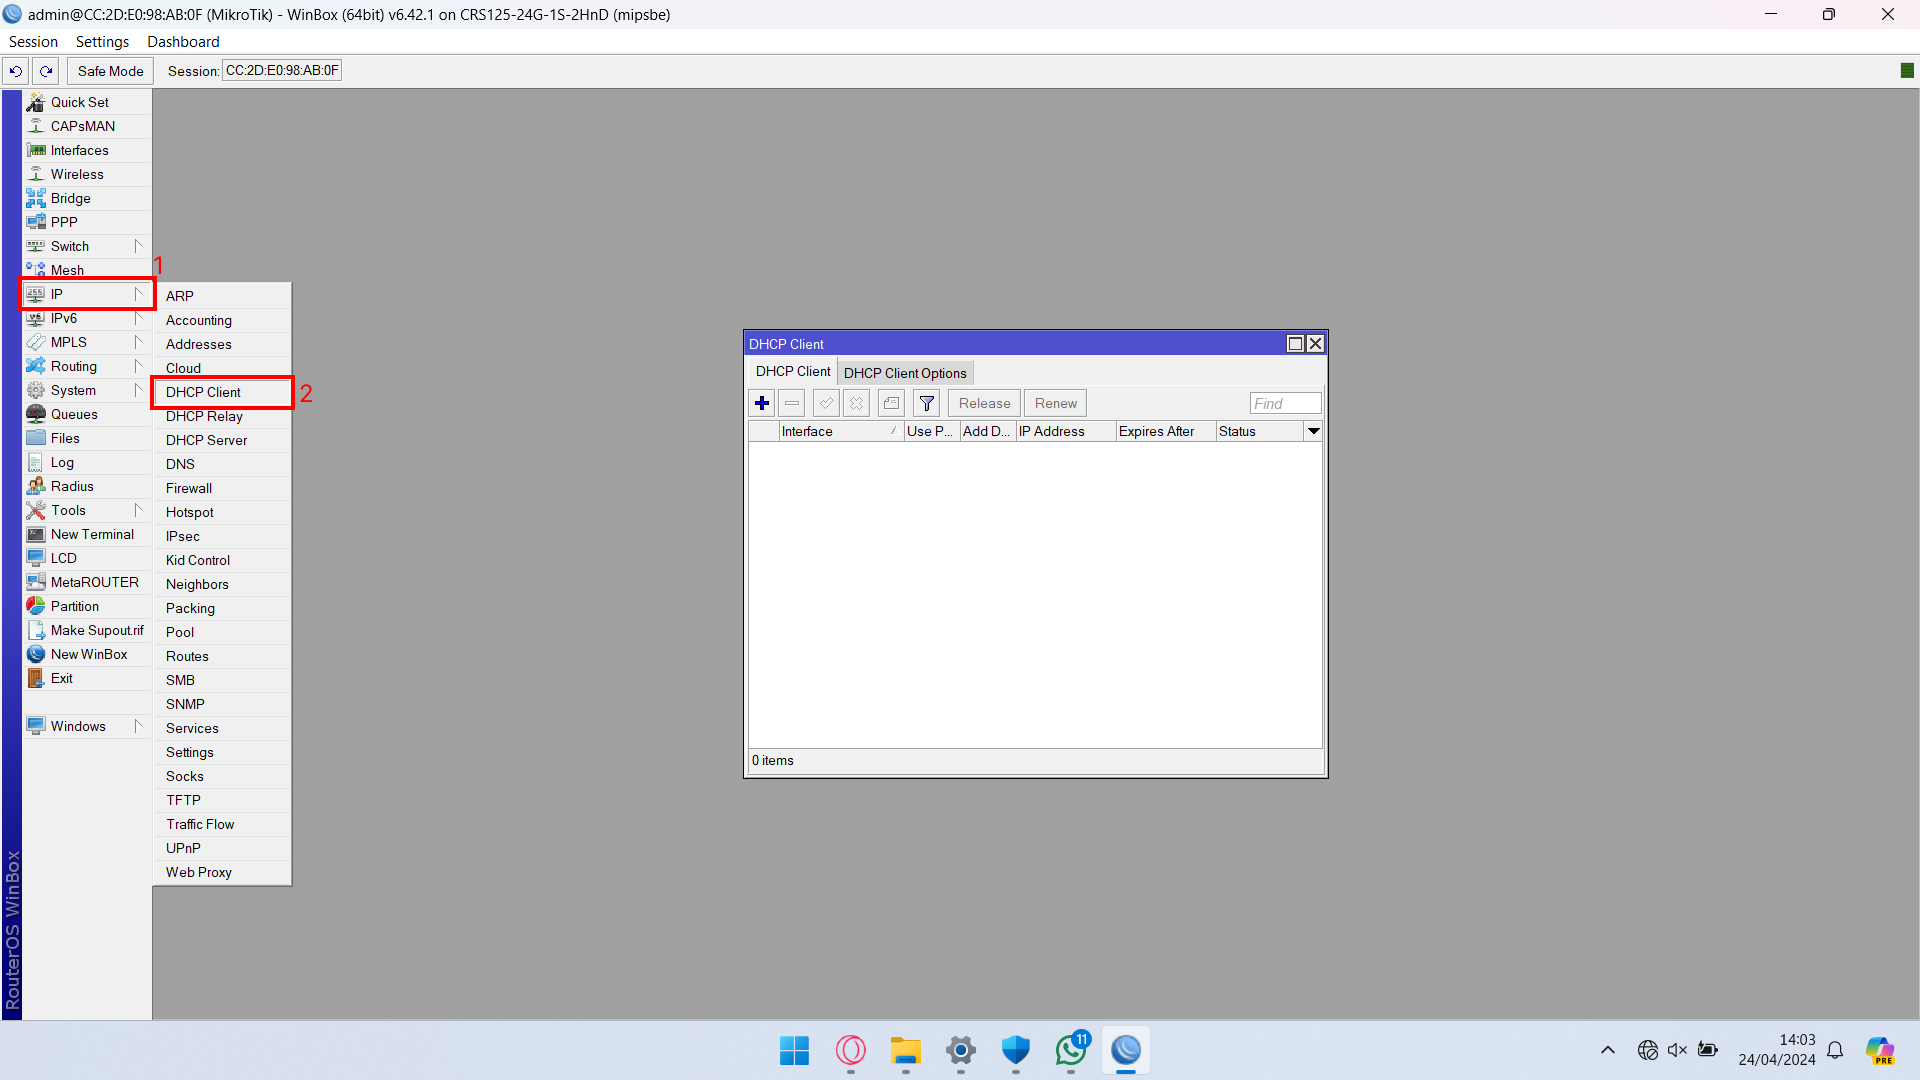
\includegraphics[width=0.5\linewidth]{P4/img/pc1/Step 2.1.png}
			\caption{Step 2.1}
			\label{fig:Step 2.1(PC 1)}
        \end{figure}
        \begin{figure}[H]
			\centering
			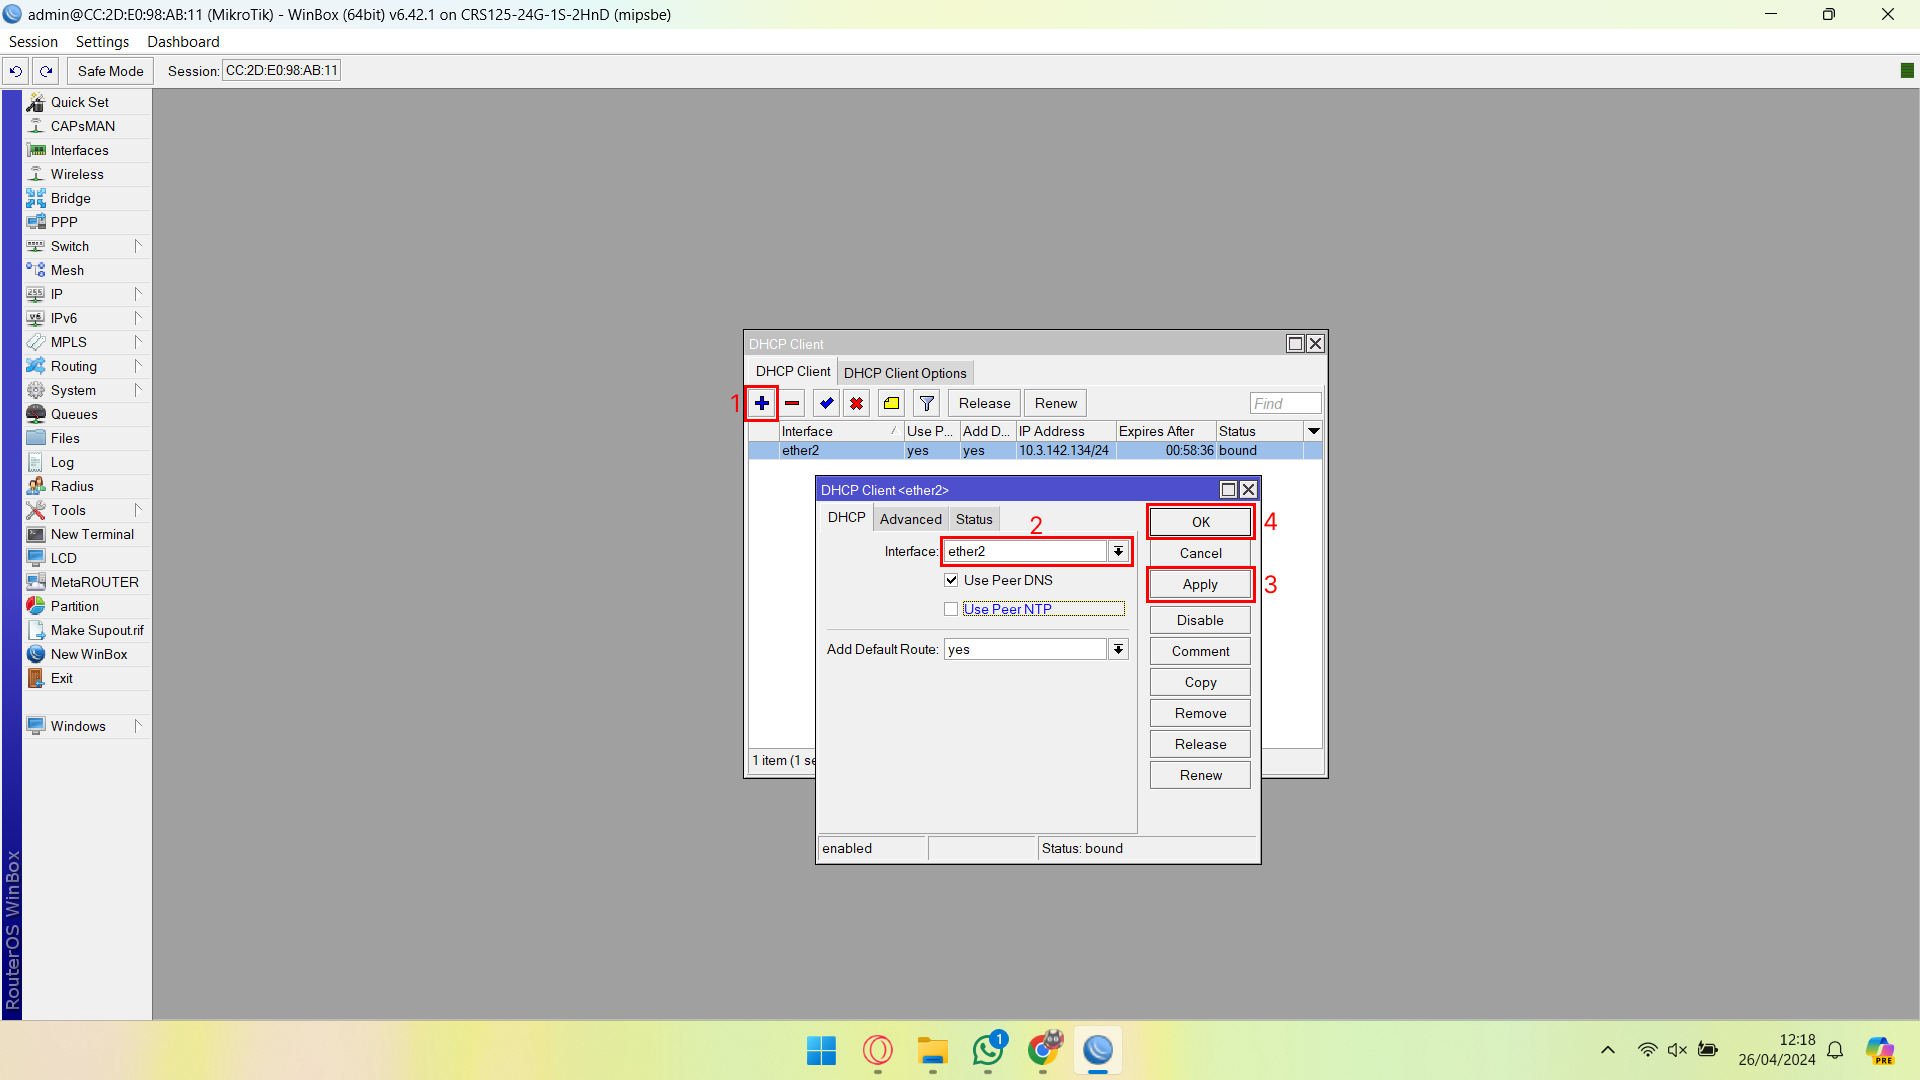
\includegraphics[width=0.8\linewidth]{P4/img/pc1/Step 2.2.png}
			\caption{Step 2.2}
			\label{fig:Step 2.2(PC 1)}
		\end{figure}
        \item Buat IP address baru pada Router 1 untuk menghubungkan PC 1 dengan Router 1. Tambahkan IP address > Isi address > Pilih Interface yang terhubung ke PC (ether4) > Klik Apply > Klik OK.
        \begin{figure}[H]
			\centering
			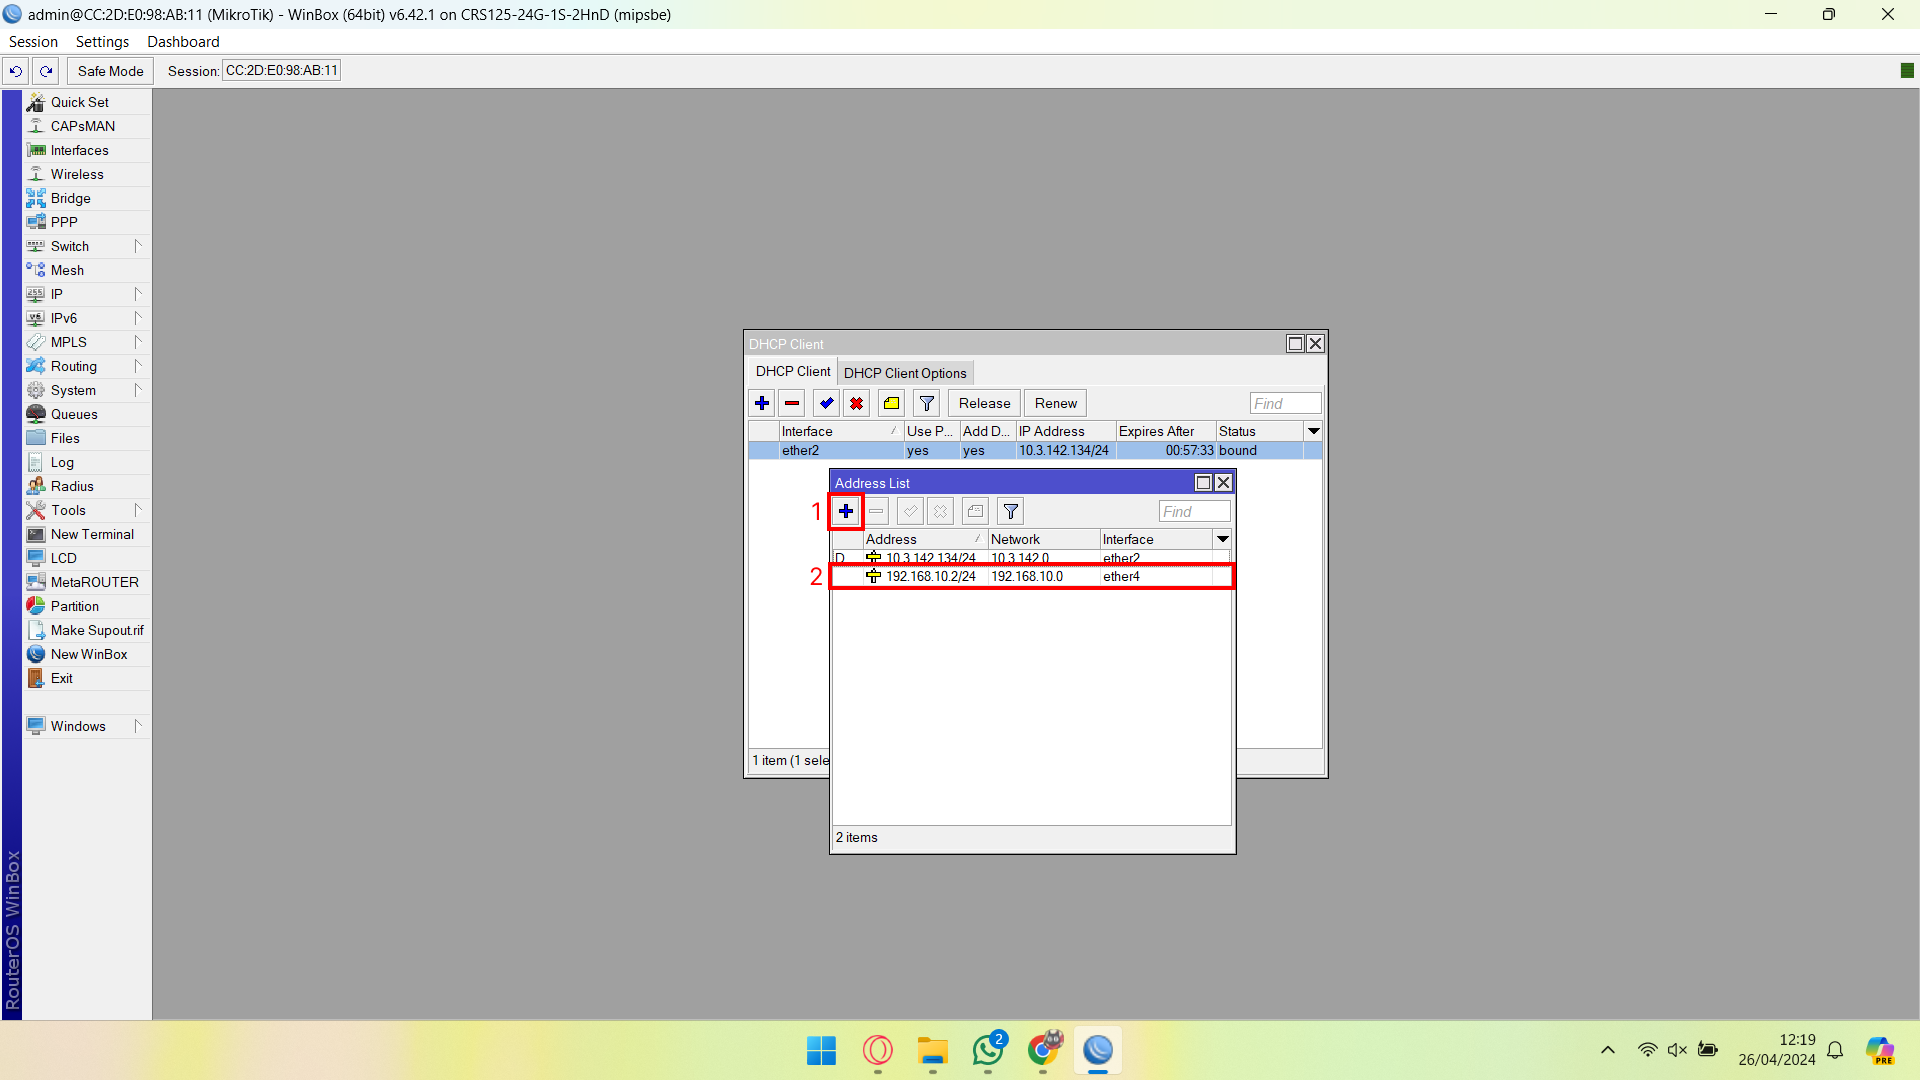
\includegraphics[width=0.8\linewidth]{P4/img/pc1/Step 3.png}
			\caption{Step 3}
			\label{fig:Step 3(PC 1)}
		\end{figure}
        \item Atur IP pada PC 1 dengan mengubah pengaturan pada setting ethernet. Ubah IP perangkat yang otomatis menjadi manual, pastikan IP PC 1 masih satu jaringan dengan IP lokal yang diinginkan, isi Gateway dengan IP address Router 1 yang tersambung dengan PC 1. Berikan IP address yang berbeda dengan contoh yang ada di modul.
        \begin{figure}[H]
			\centering
			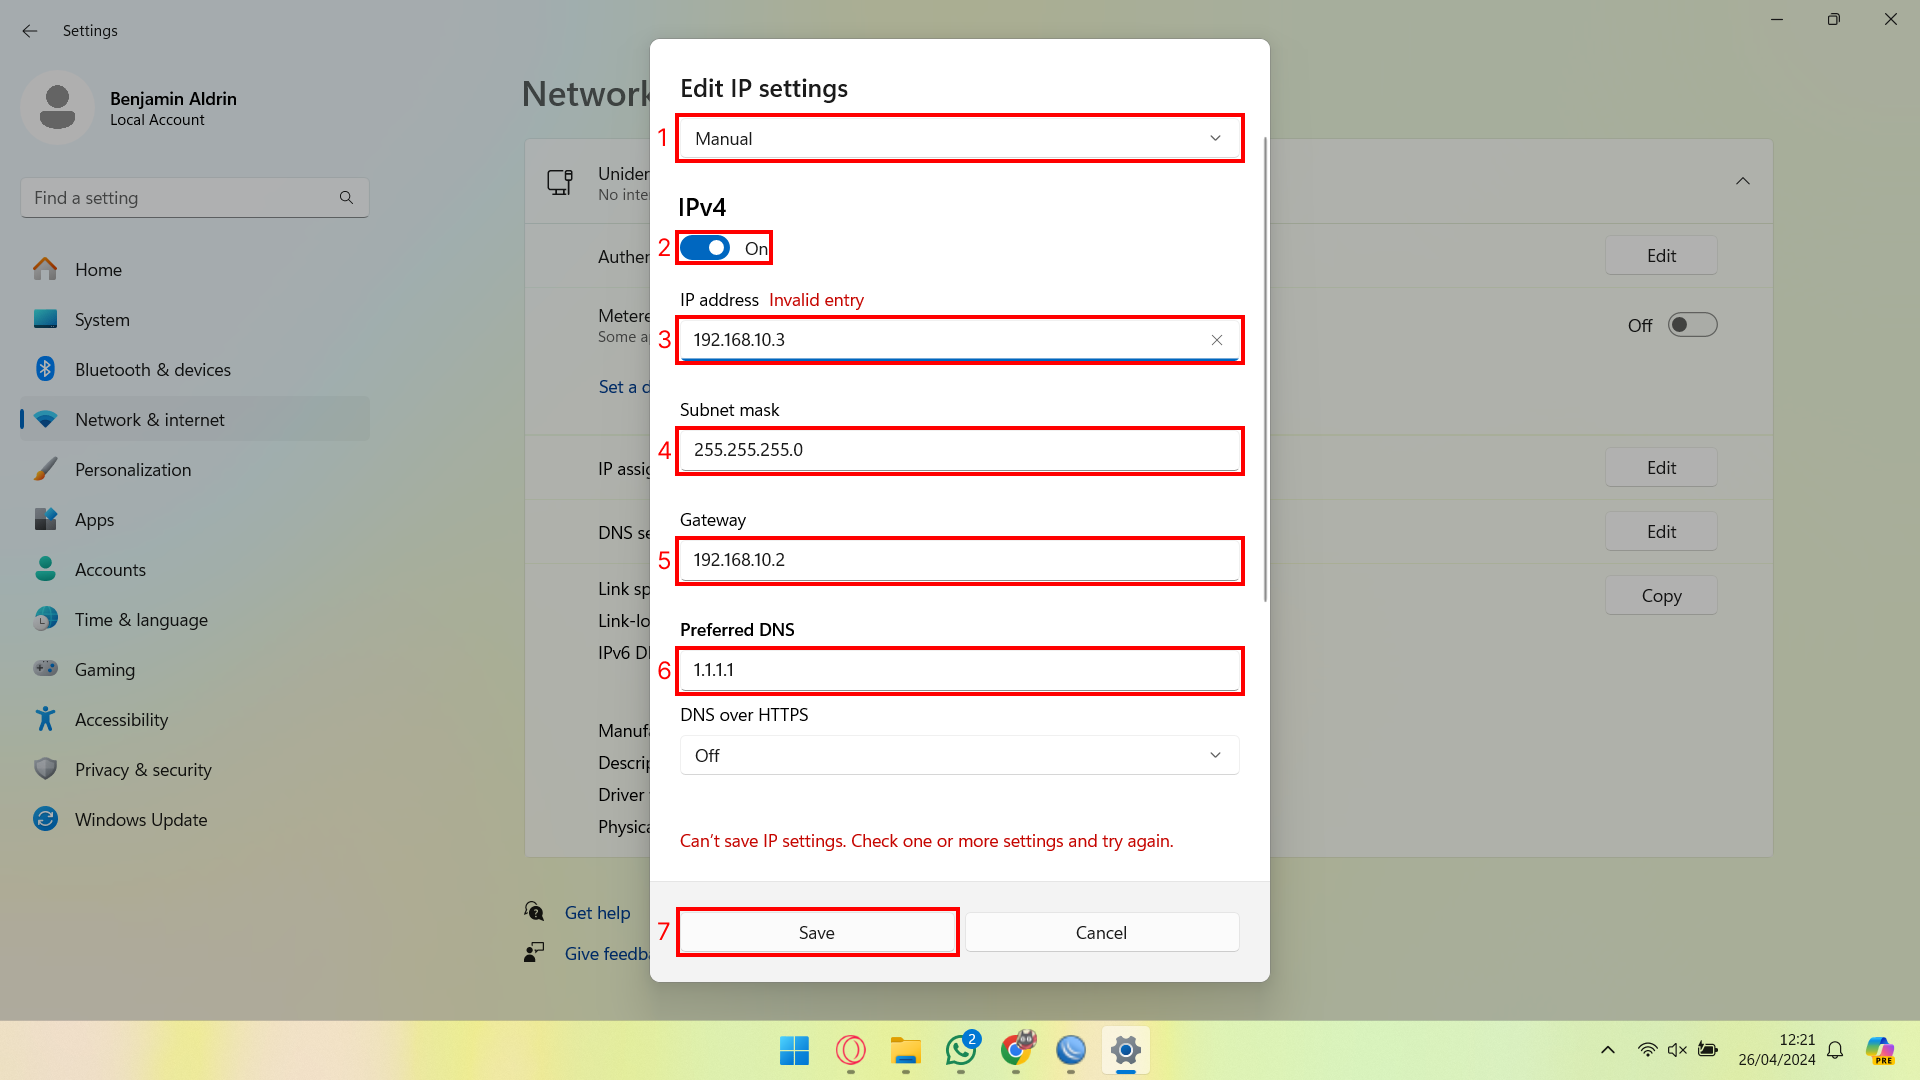
\includegraphics[width=0.8\linewidth]{P4/img/pc1/Step 4.png}
			\caption{Step 4}
			\label{fig:Step 4(PC 1)}
		\end{figure}
        \item Lakukan tes ping antara Router dengan PC1, untuk memastikan PC1 dan Router sudah terkoneksi.
        \begin{figure}[H]
			\centering
			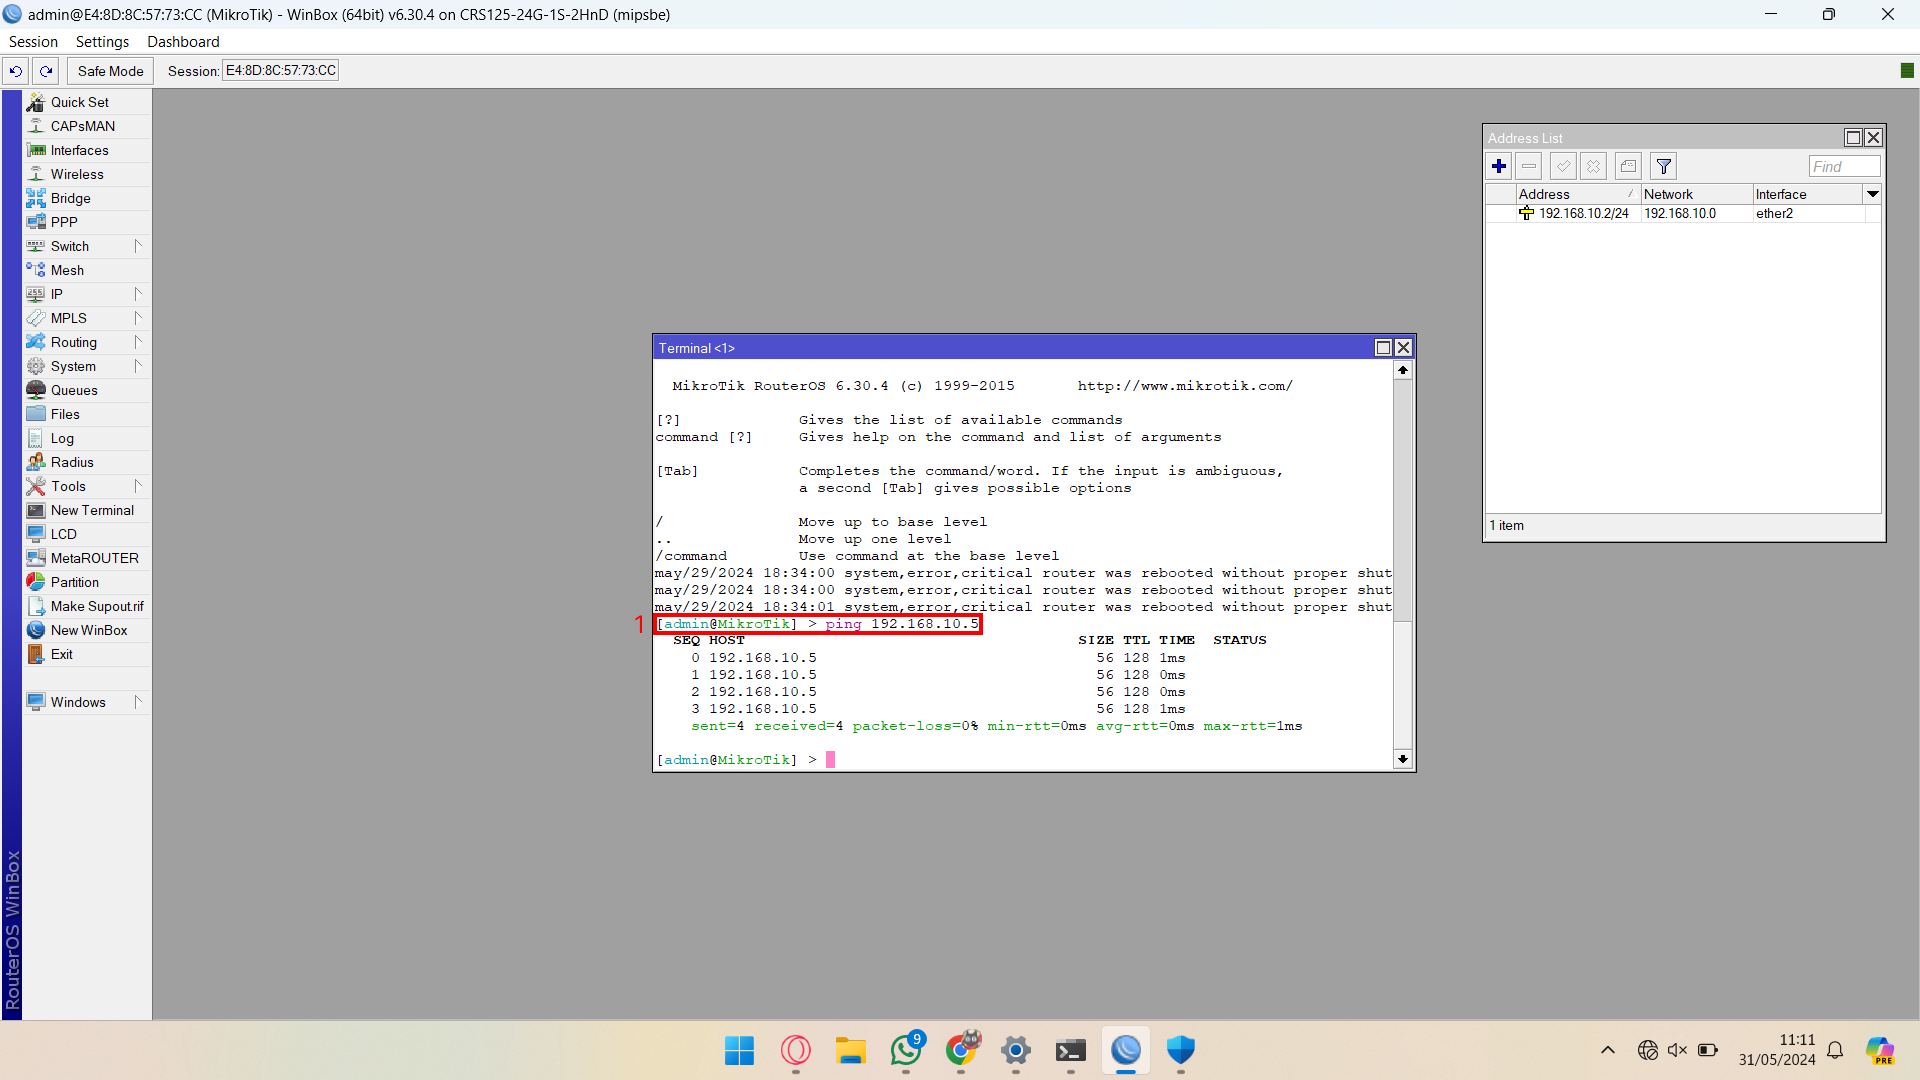
\includegraphics[width=0.8\linewidth]{P4/img/pc1/Step 5.png}
			\caption{Step 5}
			\label{fig:Step 5(PC 1)}
		\end{figure}
        \item Buat PPTP Server pada tab interface, dengan Default Profile “default -encryption”.
        \begin{figure}[H]
			\centering
			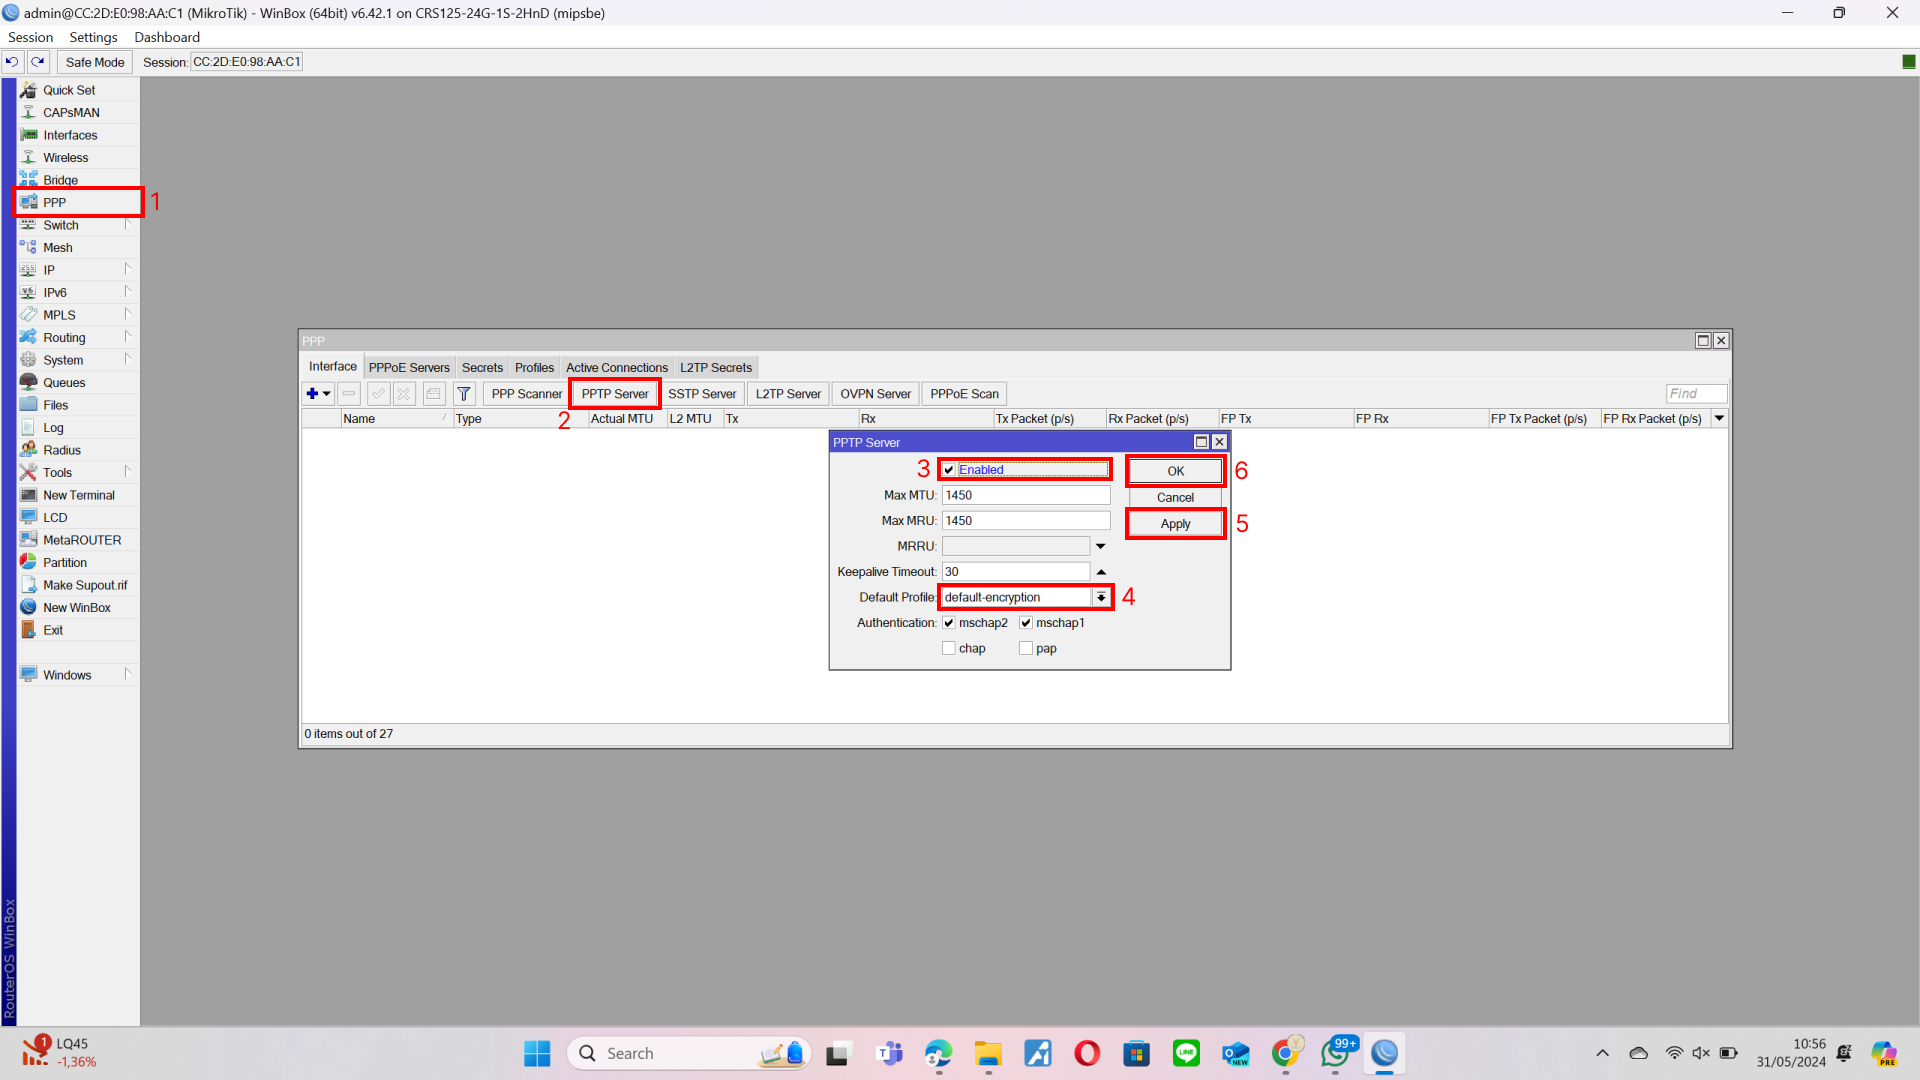
\includegraphics[width=0.8\linewidth]{P4/img/pc1/Step 6.png}
			\caption{Step 6}
			\label{fig:Step 6(PC 1)}
		\end{figure}
        \item Buat PPTP untuk client pada tab Secret, dengan konfigurasi Nama “PPTP”, Password “123456”, Service “pptp”, Profile “default”. Local Address adalah IP address tunnel pada sisi server, diisi dengan “10.10.10.2”. Remote Address adalah IP yang akan Client dapatkan, diisi dengan “10.10.10.3”. Pastikan Local Address dan Remote Address berada pada satu jaringan yang sama.
        \begin{figure}[H]
			\centering
			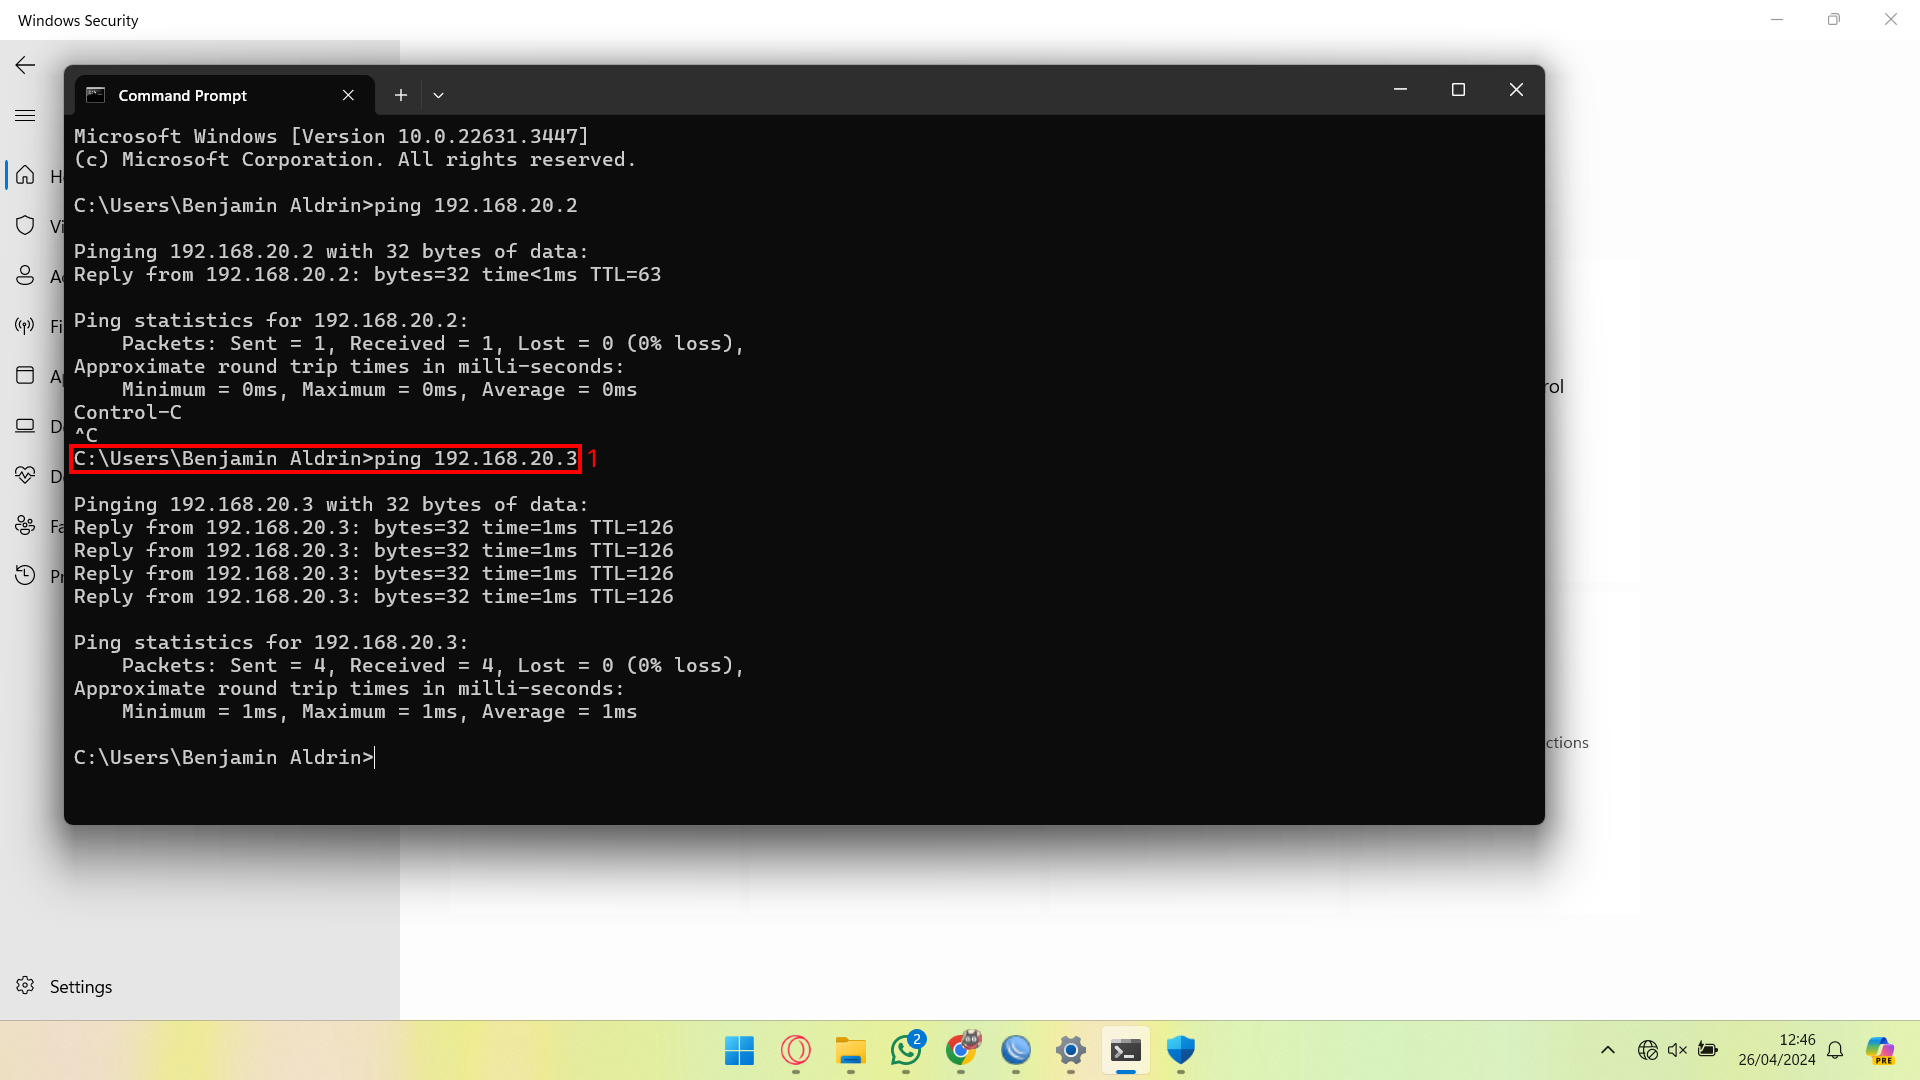
\includegraphics[width=0.8\linewidth]{P4/img/pc1/Step 7.png}
			\caption{Step 7}
			\label{fig:Step 7(PC 1)}
		\end{figure}
        \item Lakukan routing statis untuk menghubungkan PC1 dengan Internet. Buka pada tab IP > Routes, lalu tambahkan jaringan. Masukkan alamat jaringan yang ingin dituju, melalui alamat Gateway pada router 1
        \begin{figure}[H]
			\centering
			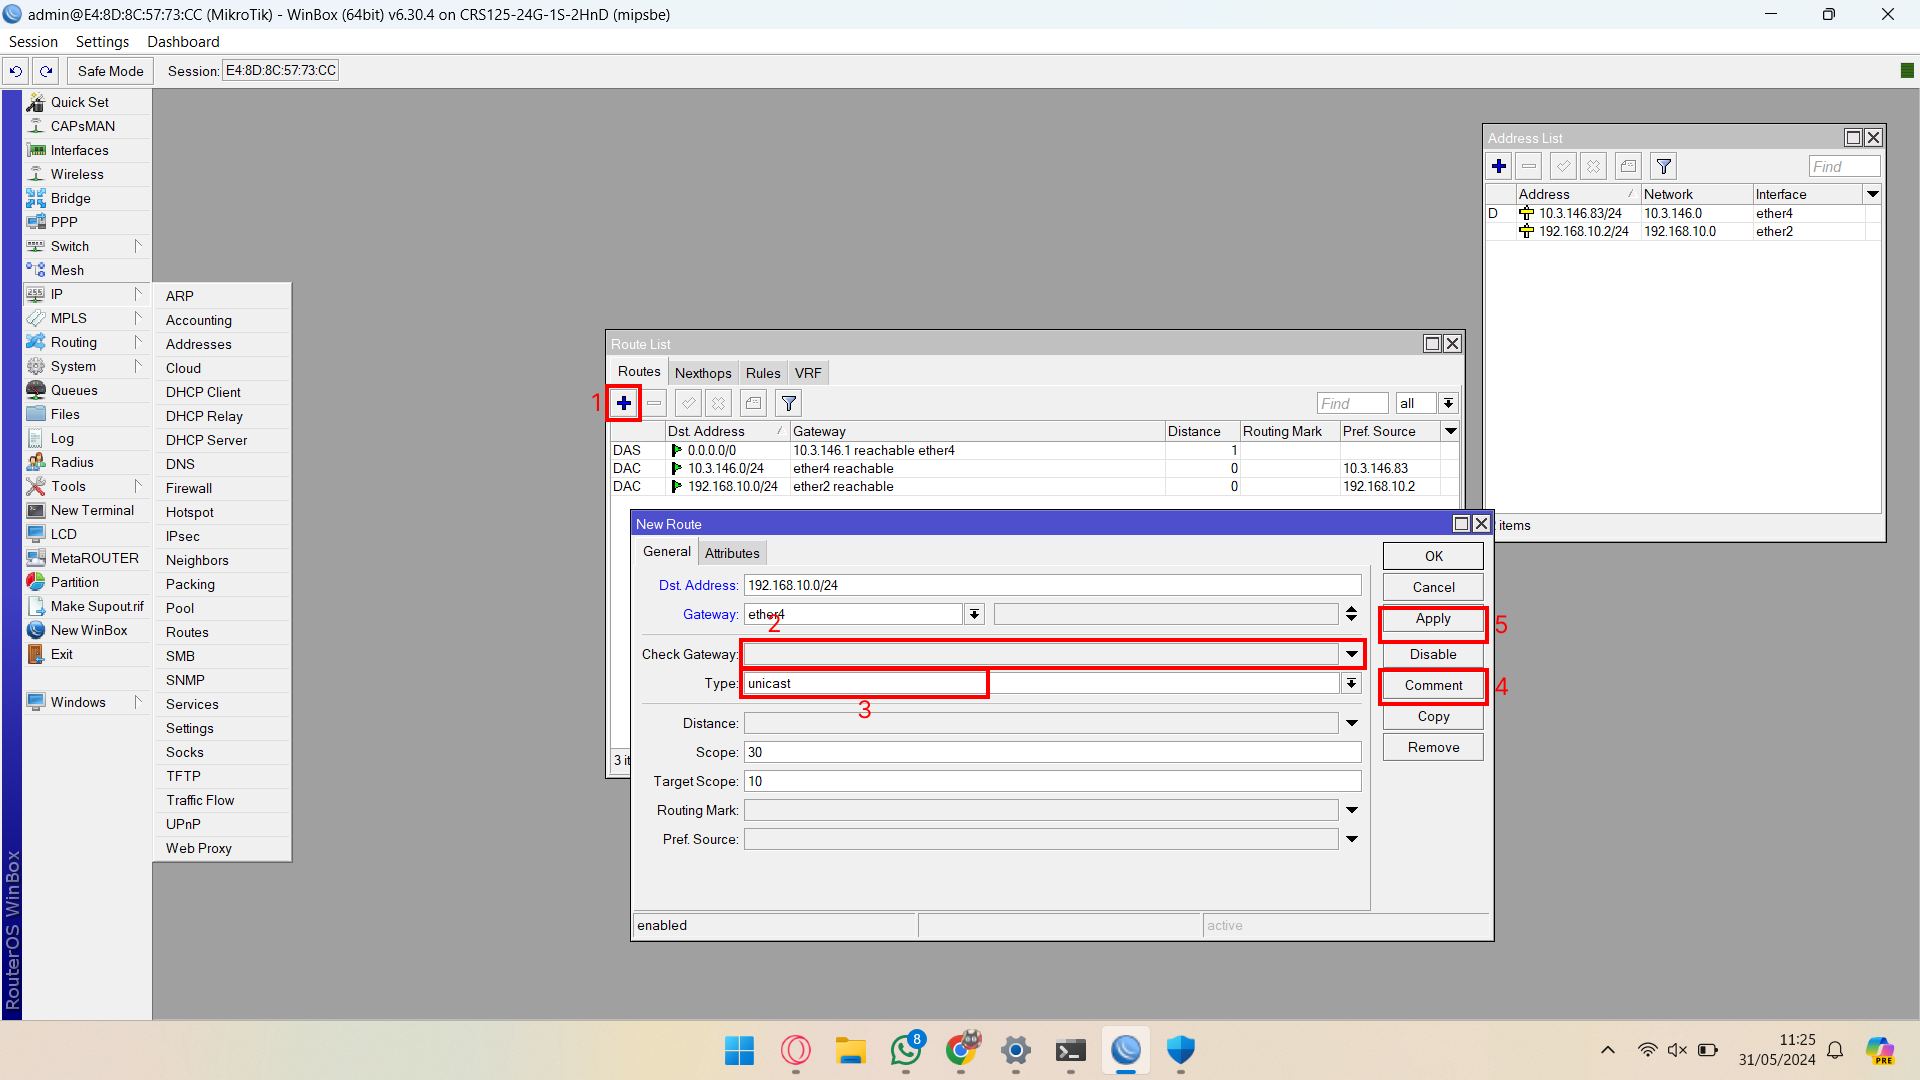
\includegraphics[width=0.8\linewidth]{P4/img/pc1/Step 8.png}
			\caption{Step 8}
			\label{fig:Step 8(PC 1)}
		\end{figure}
		\item Agar PC yang berada pada jaringan lokal dapat terhubung ke jaringan publik, dapat digunakan layanan NAT (Network Address Translation) yang akan menerjemahkan IP lokal beserta port perangkat agar dapat terhubung dengan jaringan publik. IP > Klik Firewall.
        \begin{figure}[H]
			\centering
			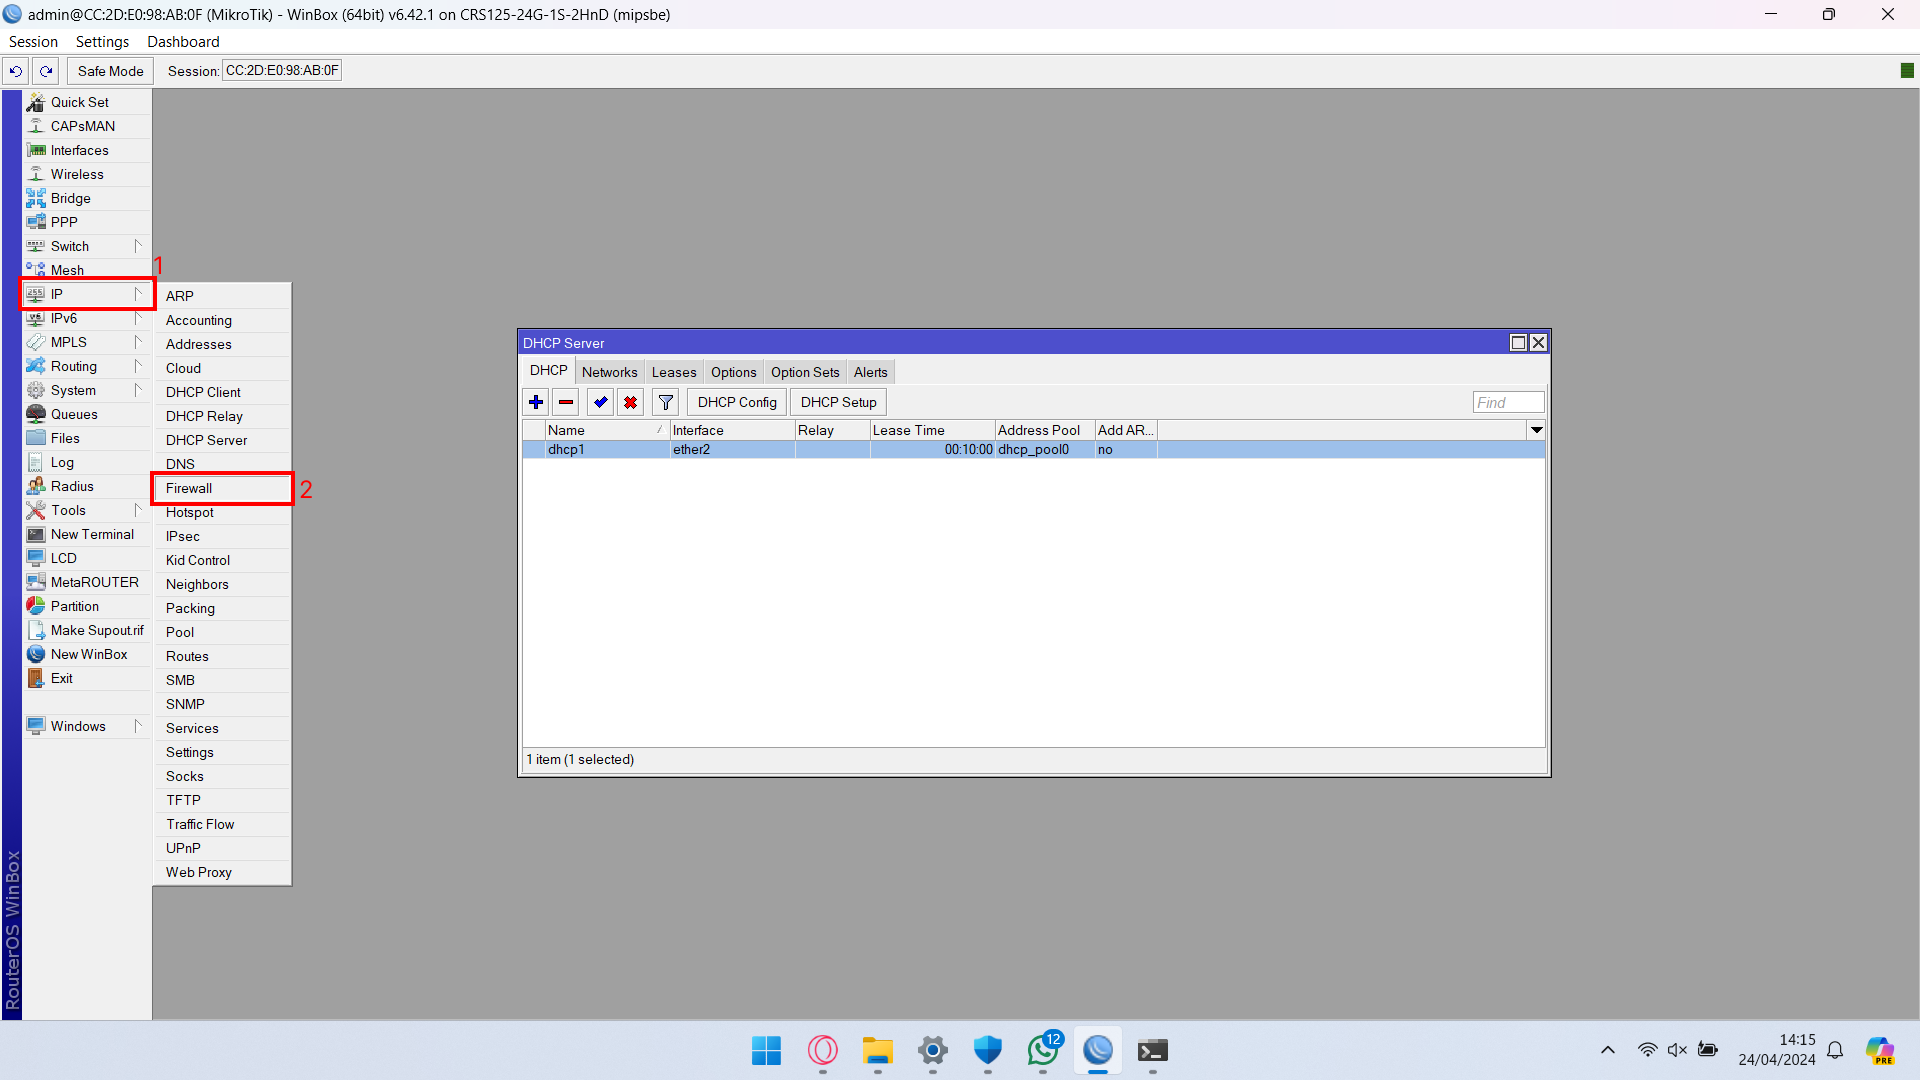
\includegraphics[width=0.8\linewidth]{P4/img/pc1/Step 16.png}
			\caption{Step 9}
			\label{fig:Step 9(PC 1)}
		\end{figure}
		\item Buat NAT baru. Klik tab NAT > Tambahkan NAT > Pada Opsi Chain pilih srcnat > Pilih Out Interface yaitu port pada Router yang terhubung dengan Internet(ether6) > Klik Apply. Tambahkan Action pada tab Action. Pada Opsi Action pilih masquerade > Klik Apply > Klik OK.
        \begin{figure}[H]
			\centering
			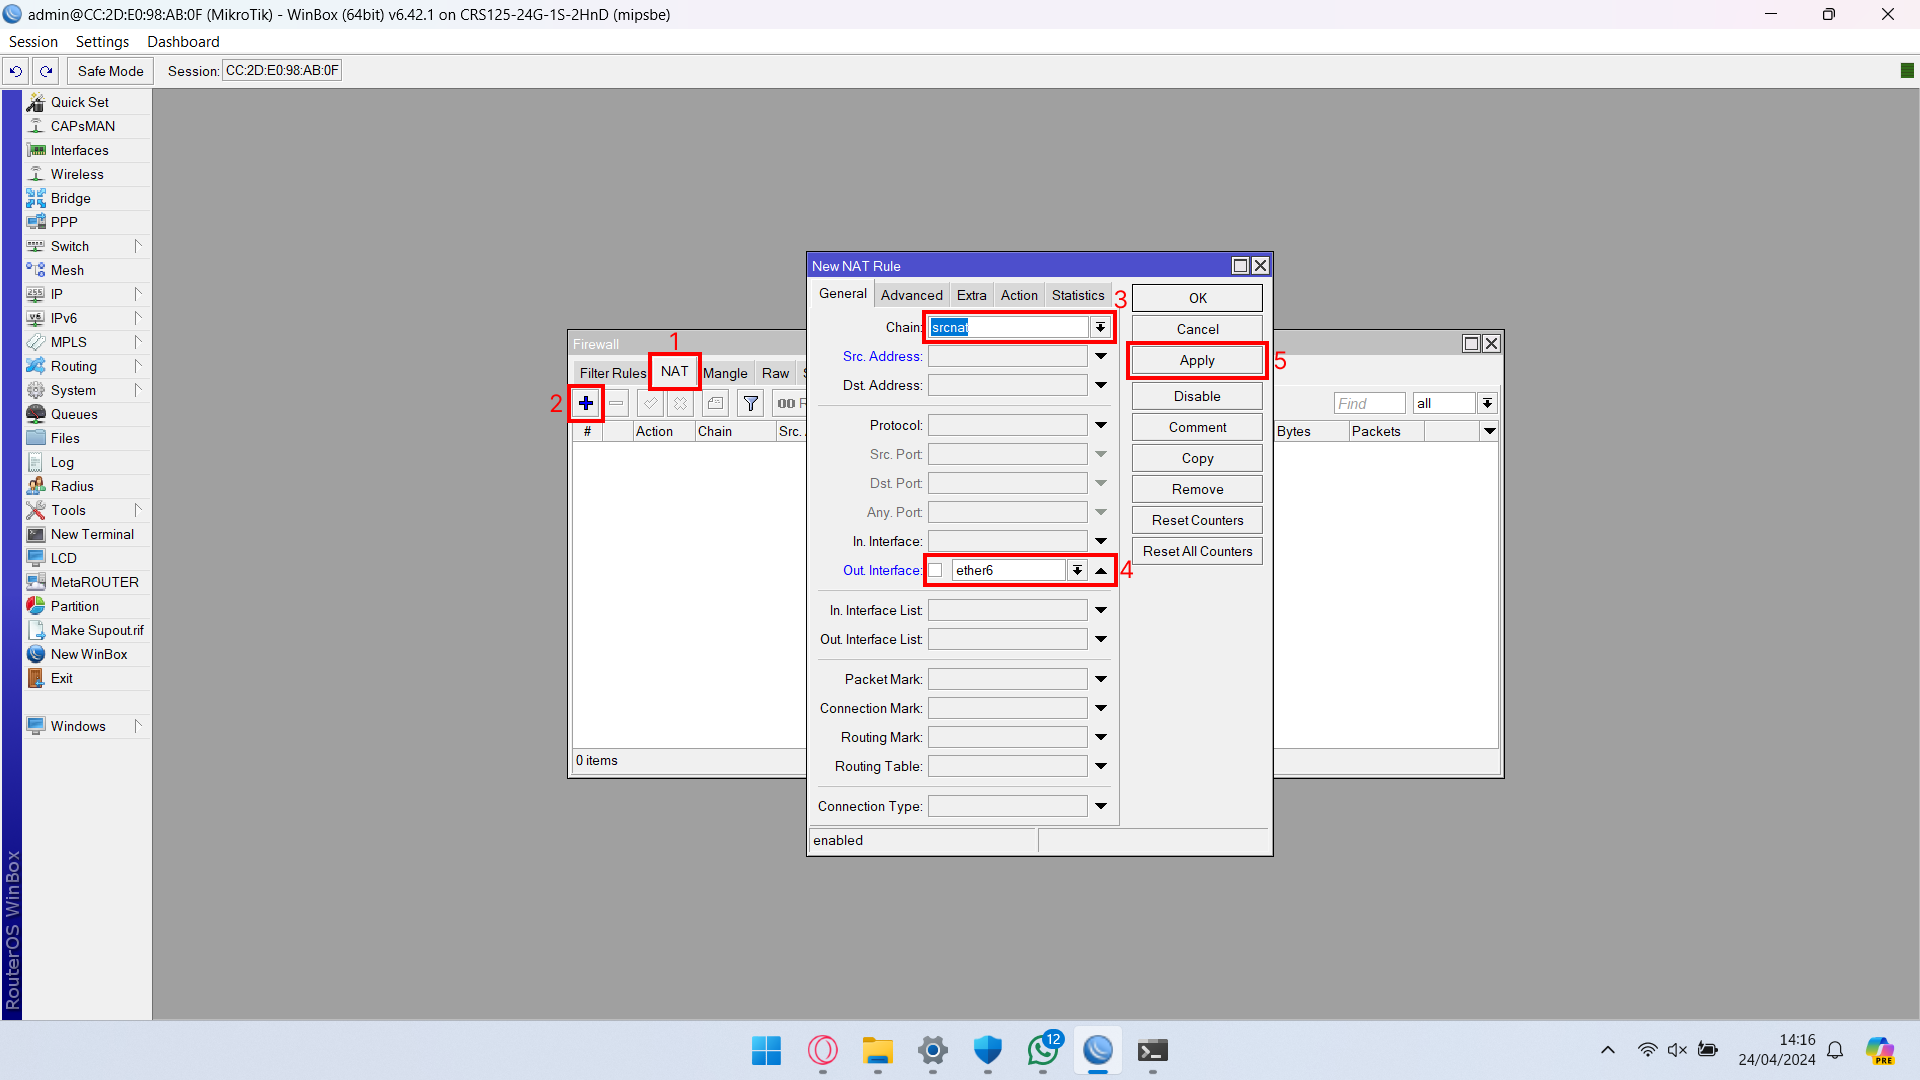
\includegraphics[width=0.5\linewidth]{P4/img/pc1/Step 15.png}
			\caption{Step 10.1}
			\label{fig:Step 10.1(PC 1)}
        \end{figure}
        \begin{figure}[H]
			\centering
			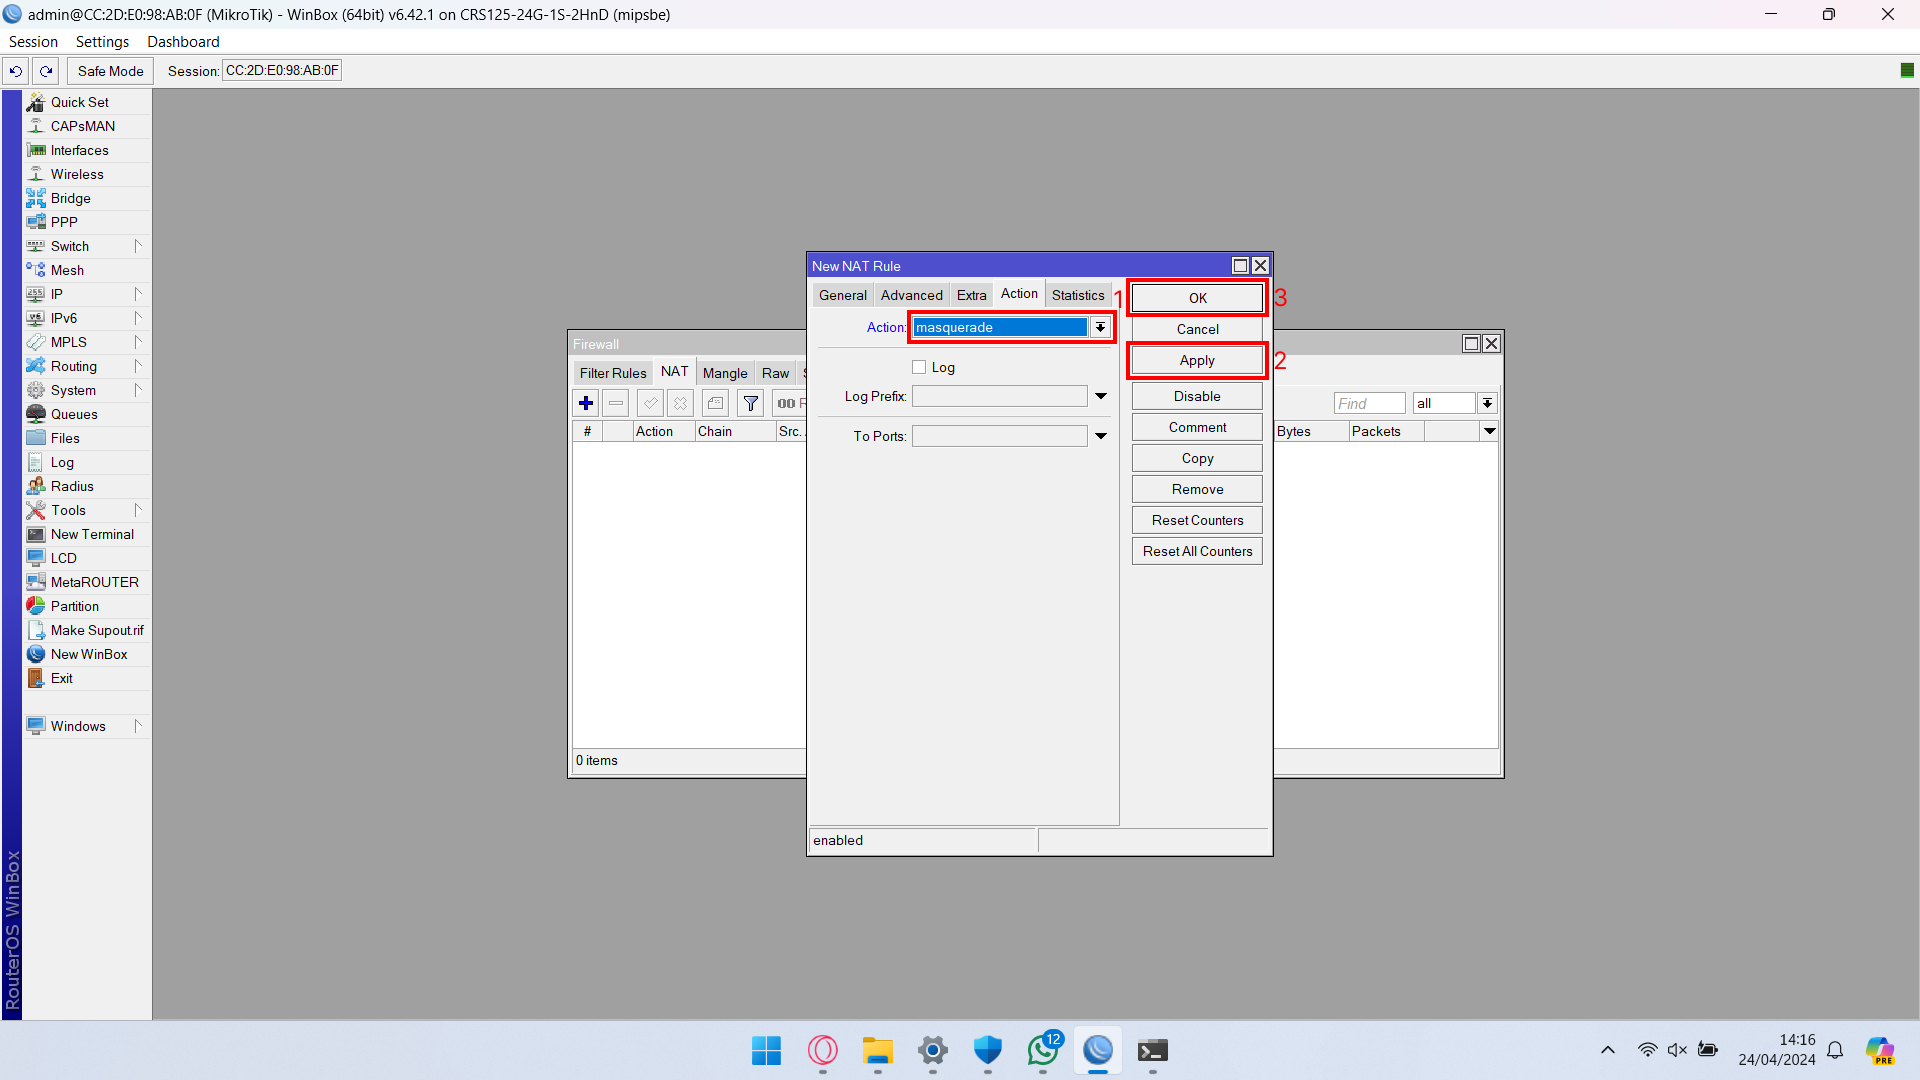
\includegraphics[width=0.8\linewidth]{P4/img/pc1/Step 14.png}
			\caption{Step 10.2}
			\label{fig:Step 10.2(PC 1)}
		\end{figure}	
    \end{enumerate}
	\textbf{Pengujian Konfigurasi}
	\begin{enumerate}
		\item Lakukan tes ping ke alamat Remote Address Router 2 untuk memastikan kedua Router sudah terhubung.
		\begin{figure}[H]
			\centering
			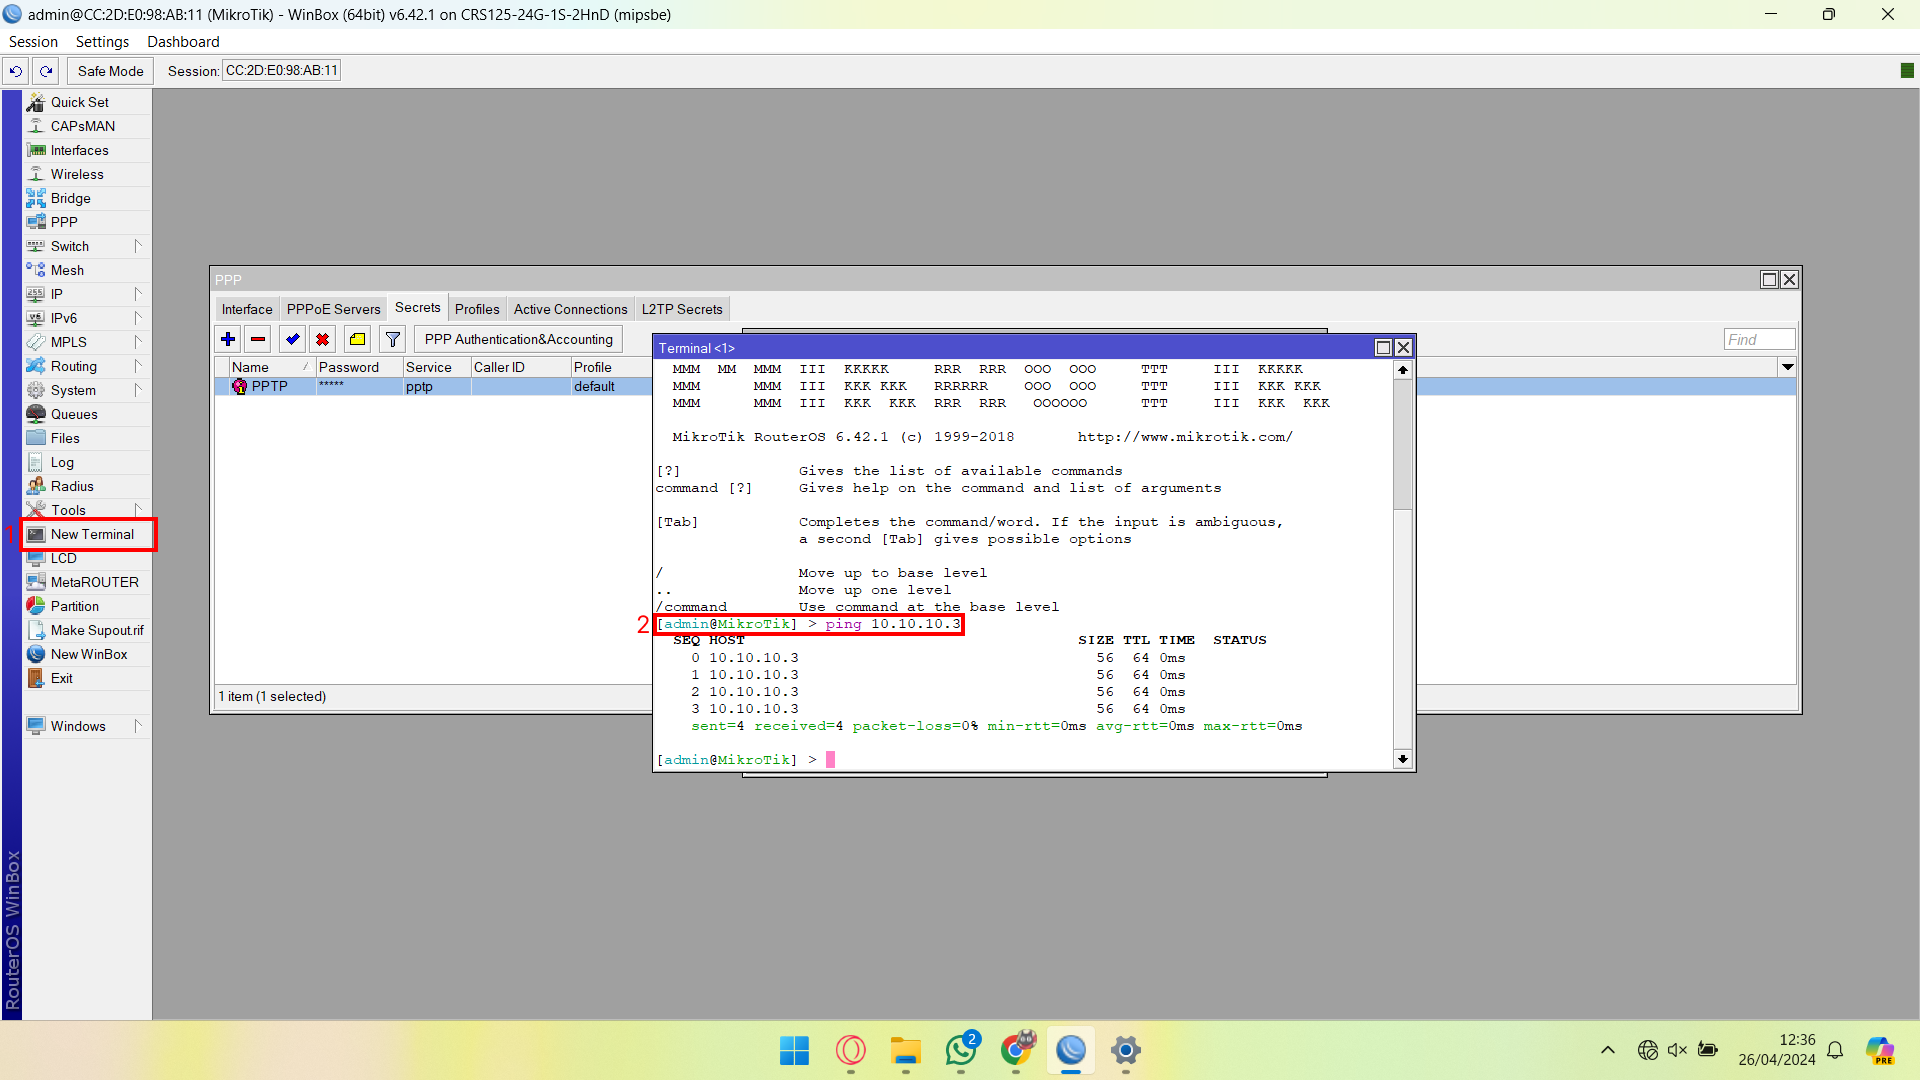
\includegraphics[width=0.8\linewidth]{P4/img/pc1/Step 9.png}
			\caption{Step 1}
			\label{fig:Ping Step 1(PC 1)}
		\end{figure}
		\item Lakukan tes ping ke PC 2 untuk memastikan kedua PC sudah terhubung.
		\begin{figure}[H]
			\centering
			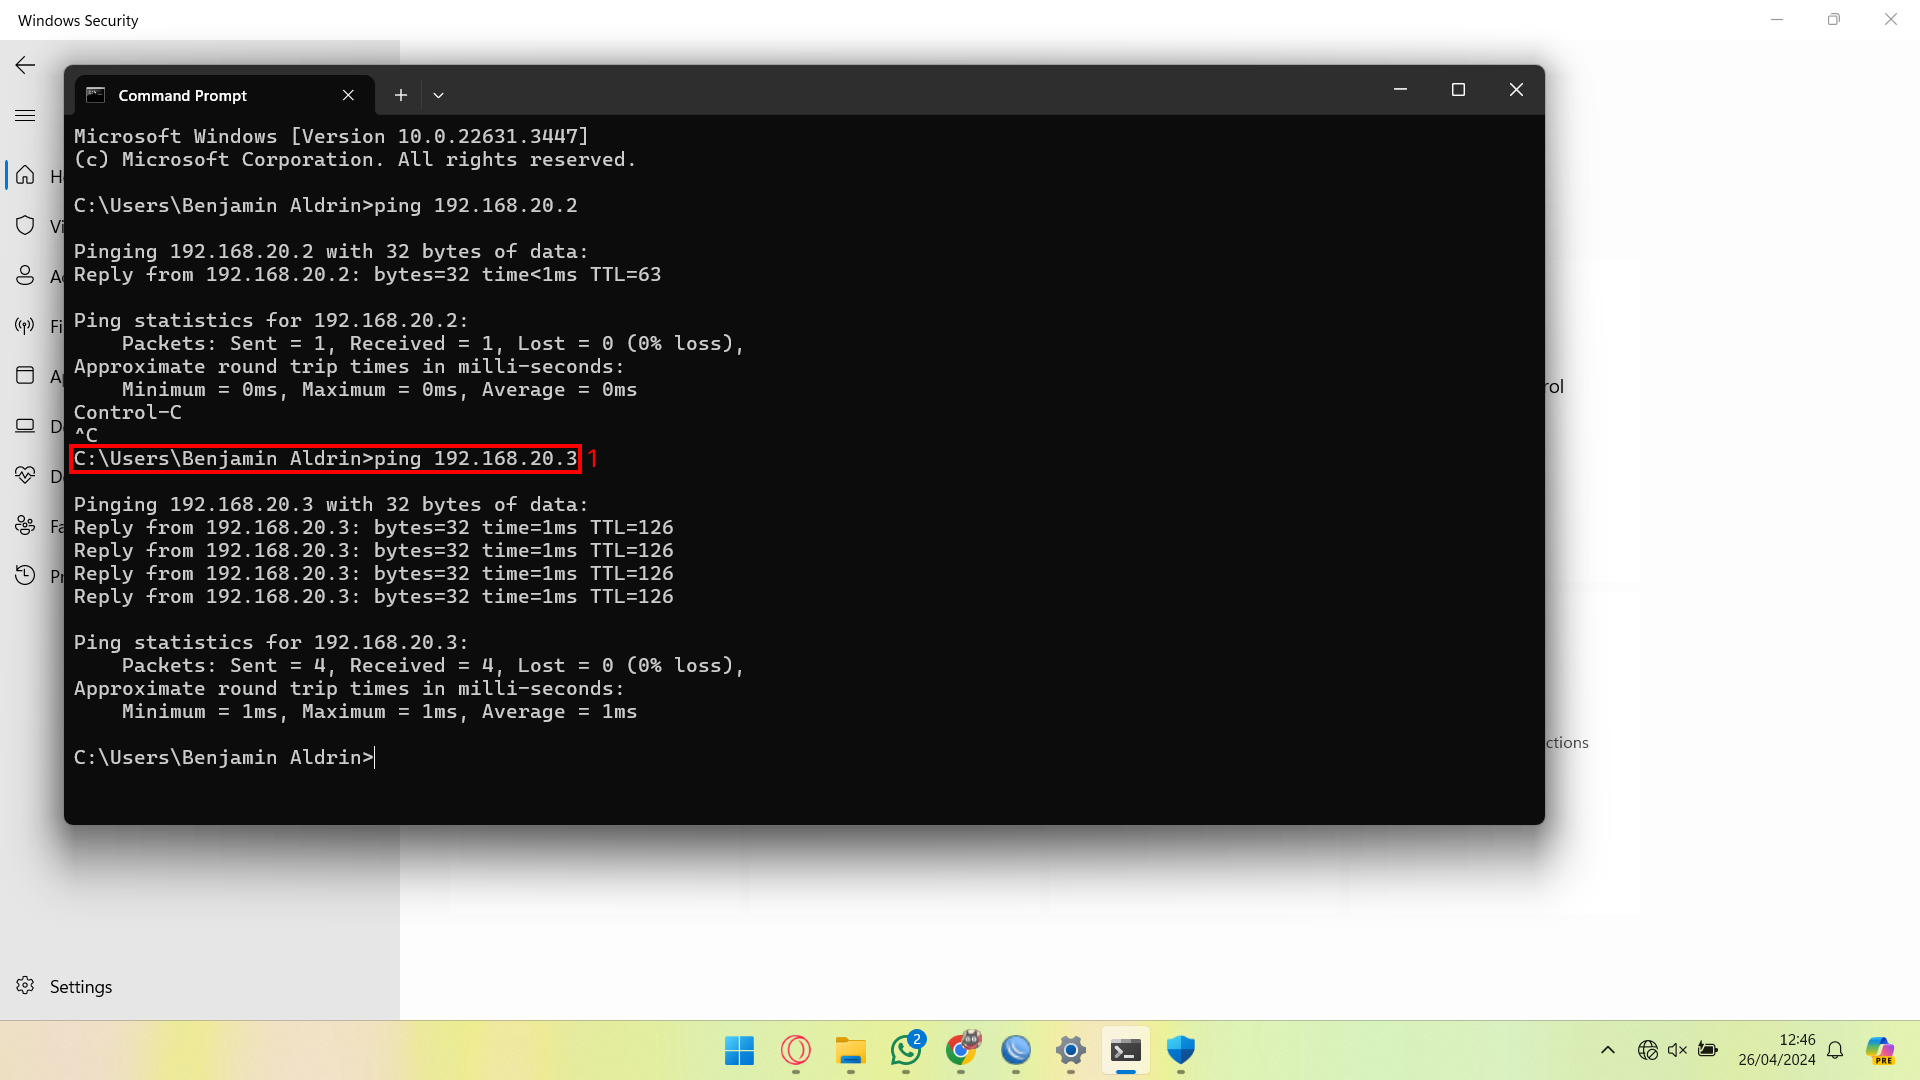
\includegraphics[width=0.8\linewidth]{P4/img/pc1/Step 10.png}
			\caption{Step 2}
			\label{fig:Ping Step 2(PC 1)}
		\end{figure}
	\end{enumerate}

    \textbf{Konfigurasi PC 2}
    \begin{enumerate}
        \item Hubungkan PC2 dengan Internet, bisa dilakukan menggunakan wifi ITS.
        \begin{figure}[H]
			\centering
			\includegraphics[width=0.5\linewidth]{P4/img/pc2/Step 1.png}
			\caption{Step 1}
			\label{fig:Step 1(PC 2)}
		\end{figure}
        \item Cek IP yang diterima PC2 dari ITS.
        \begin{figure}[H]
			\centering
			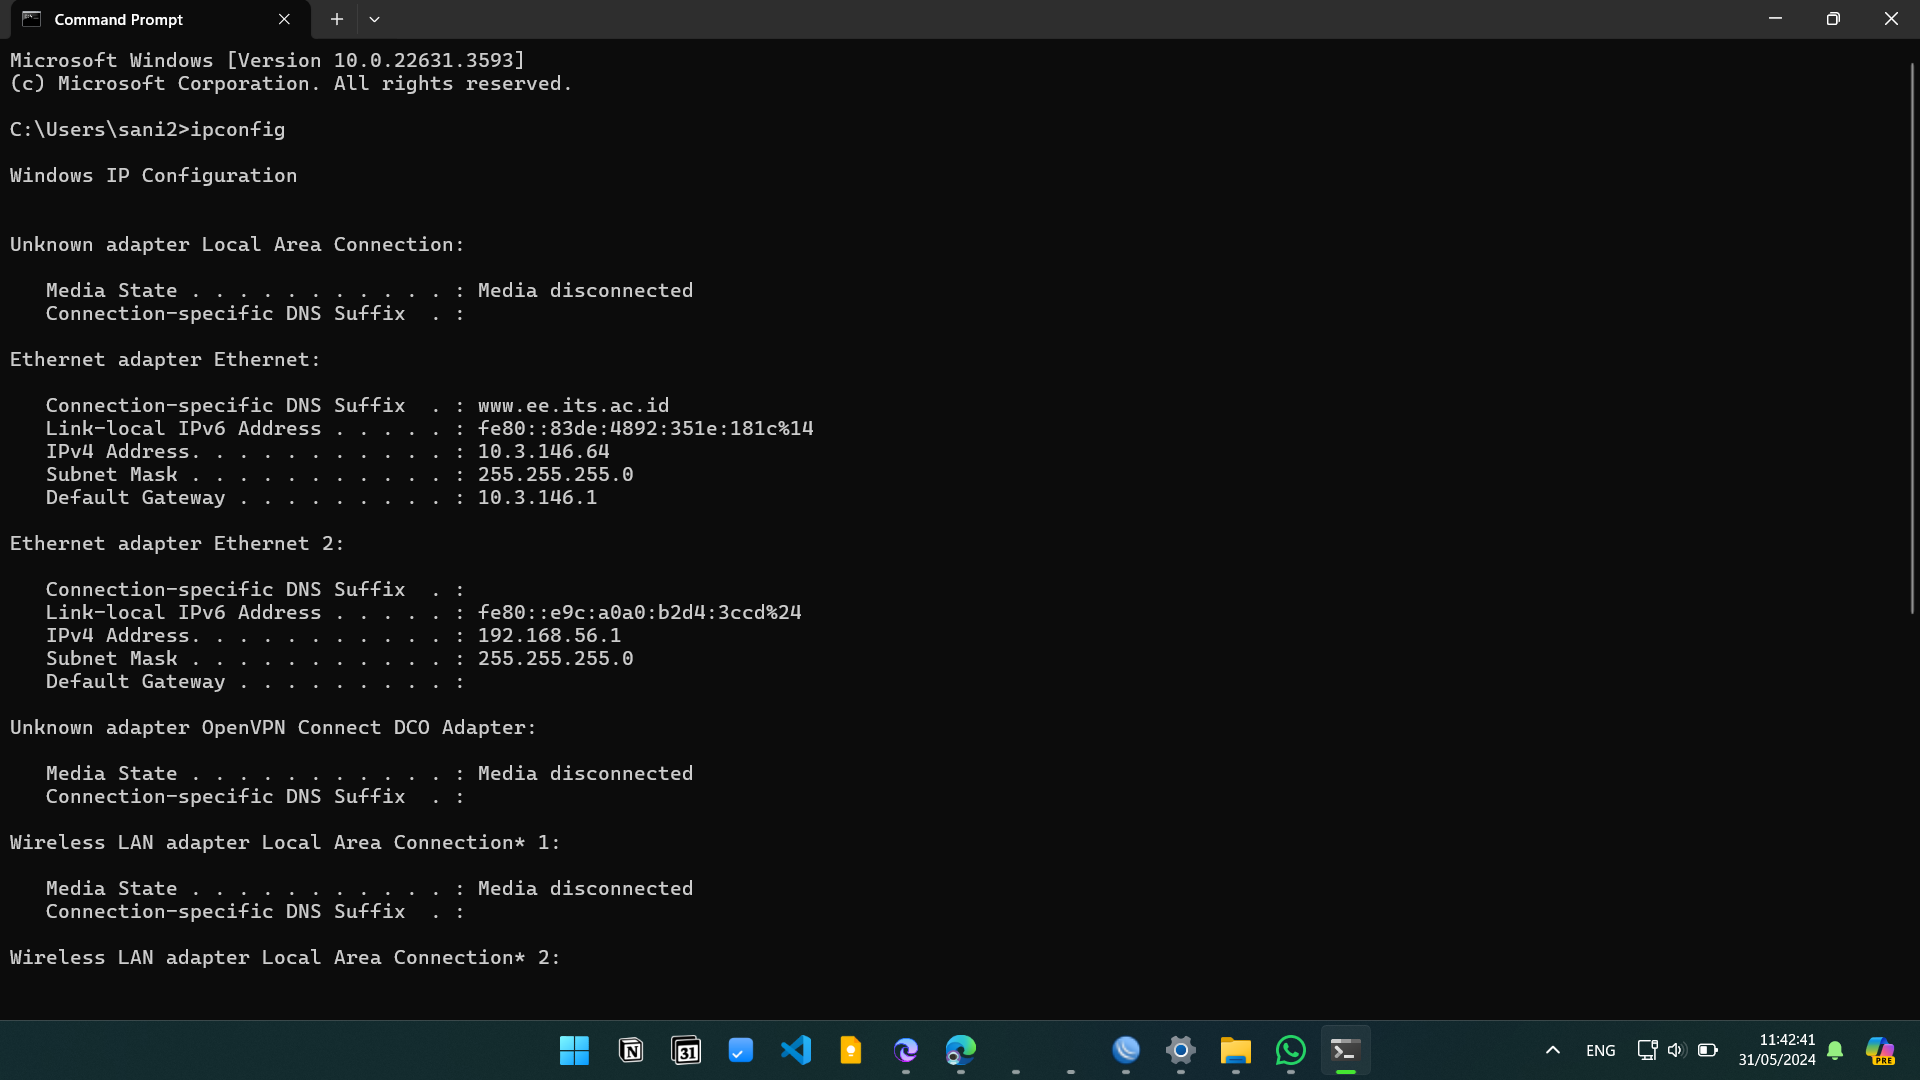
\includegraphics[width=0.5\linewidth]{P4/img/pc2/Step 2.png}
			\caption{Step 2}
			\label{fig:Step 2(PC 2)}
        \end{figure}
        \item Masuk ke dalam setting PC2 dan klik VPN.
        \begin{figure}[H]
			\centering
			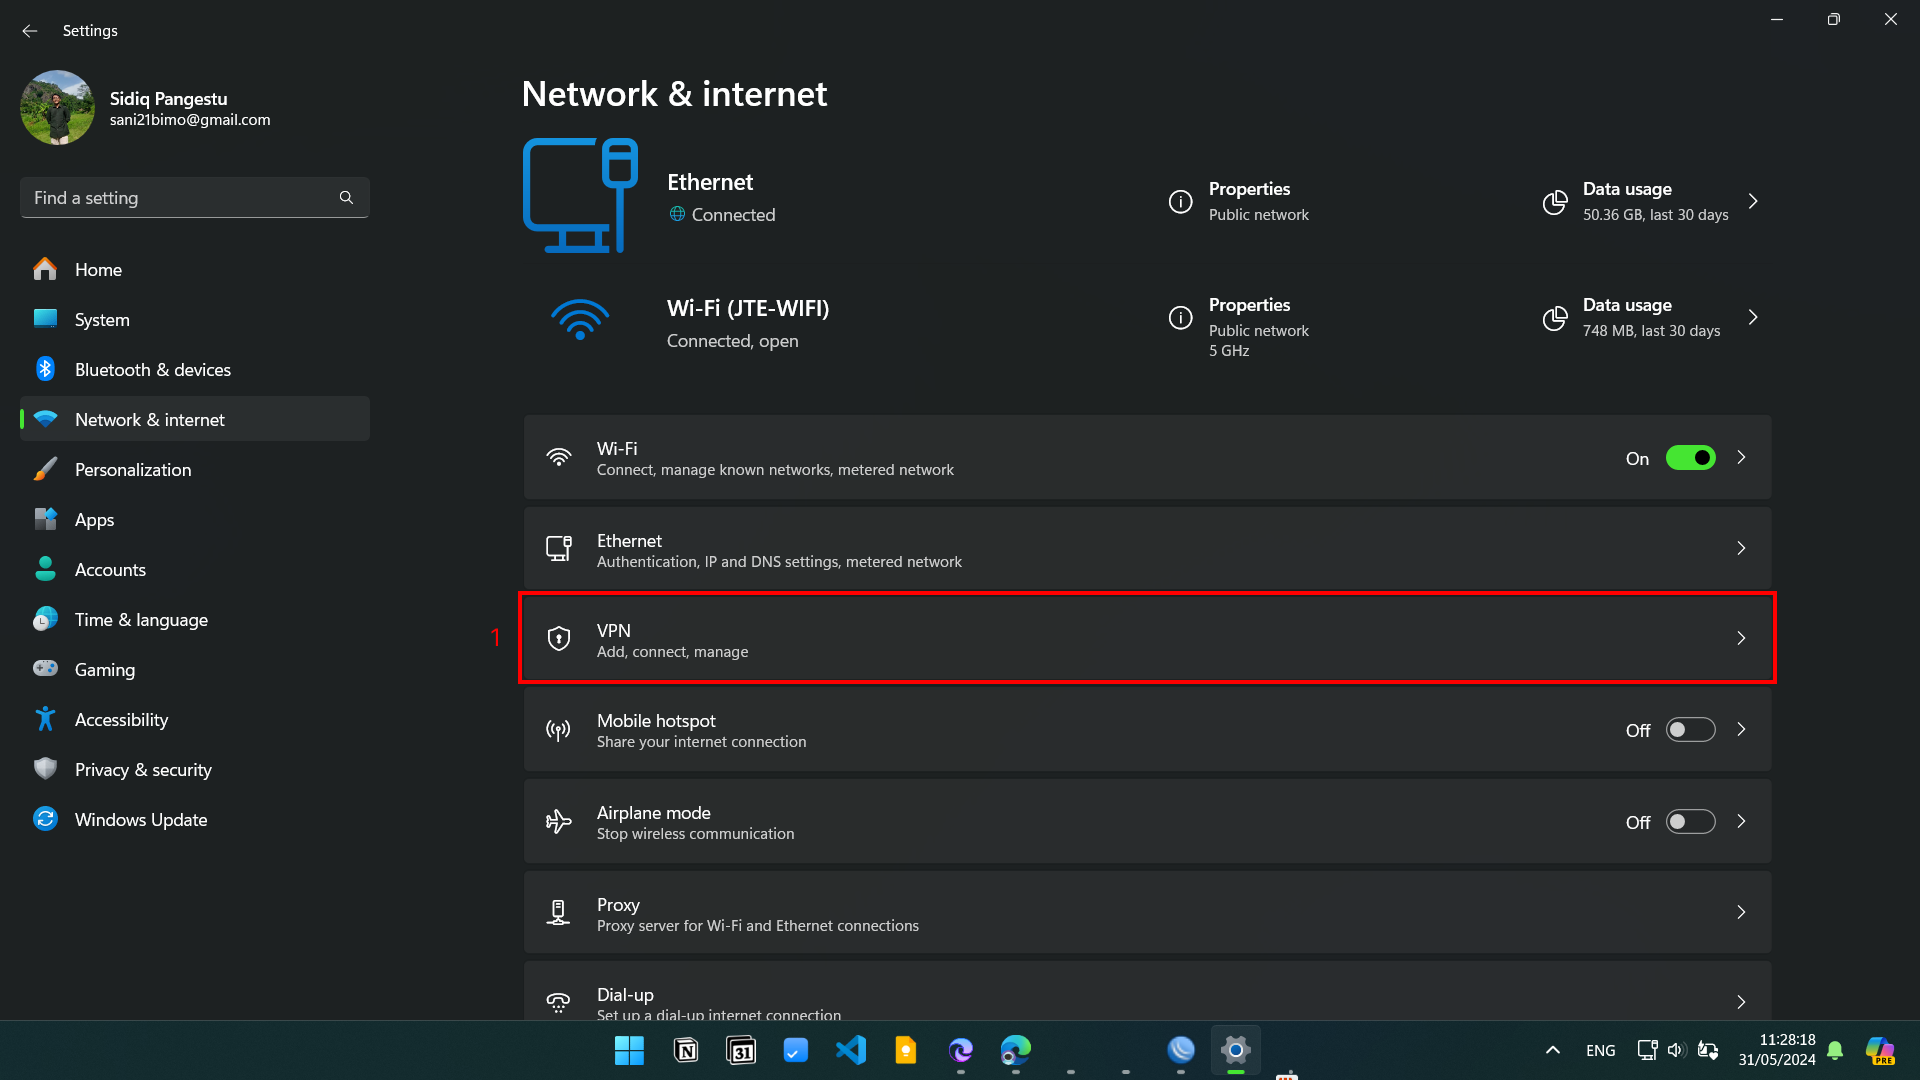
\includegraphics[width=0.8\linewidth]{P4/img/pc2/Step 3.png}
			\caption{Step 3}
			\label{fig:Step 3(PC 2)}
		\end{figure}
        \item Hubungkan client PPTP dengan server PPTP, untuk melakukan hal tersebut, buatlah koneksi VPN baru antara PC2 dengan Host Server. Pastikan menggunakan VPN type PPTP. Pastikan Username dan password sudah sesuai dengan konfigurasi Router1.
        \begin{figure}[H]
			\centering
			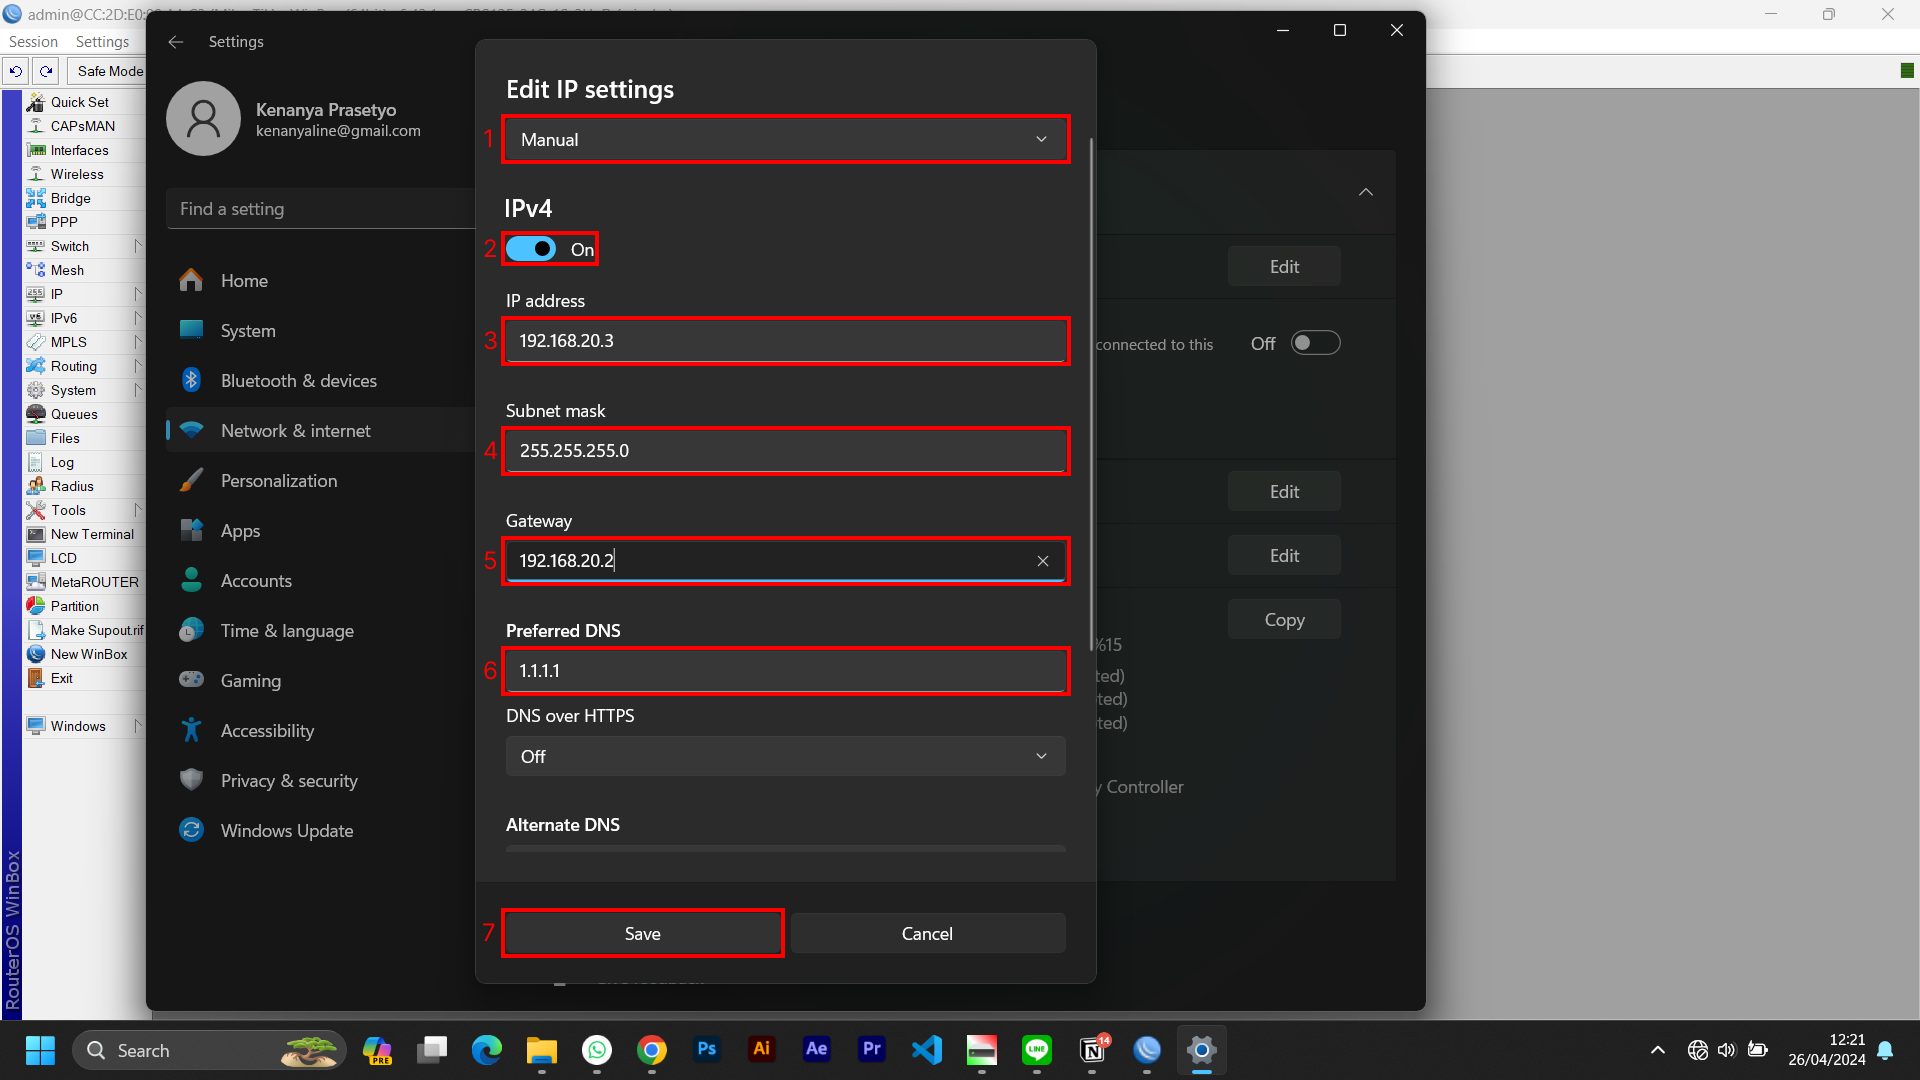
\includegraphics[width=0.8\linewidth]{P4/img/pc2/Step 4.png}
			\caption{Step 4}
			\label{fig:Step 4(PC 2)}
		\end{figure}
        \item Hubungkan ke VPN dengan cara klik tombol Connect
        \begin{figure}[H]
			\centering
			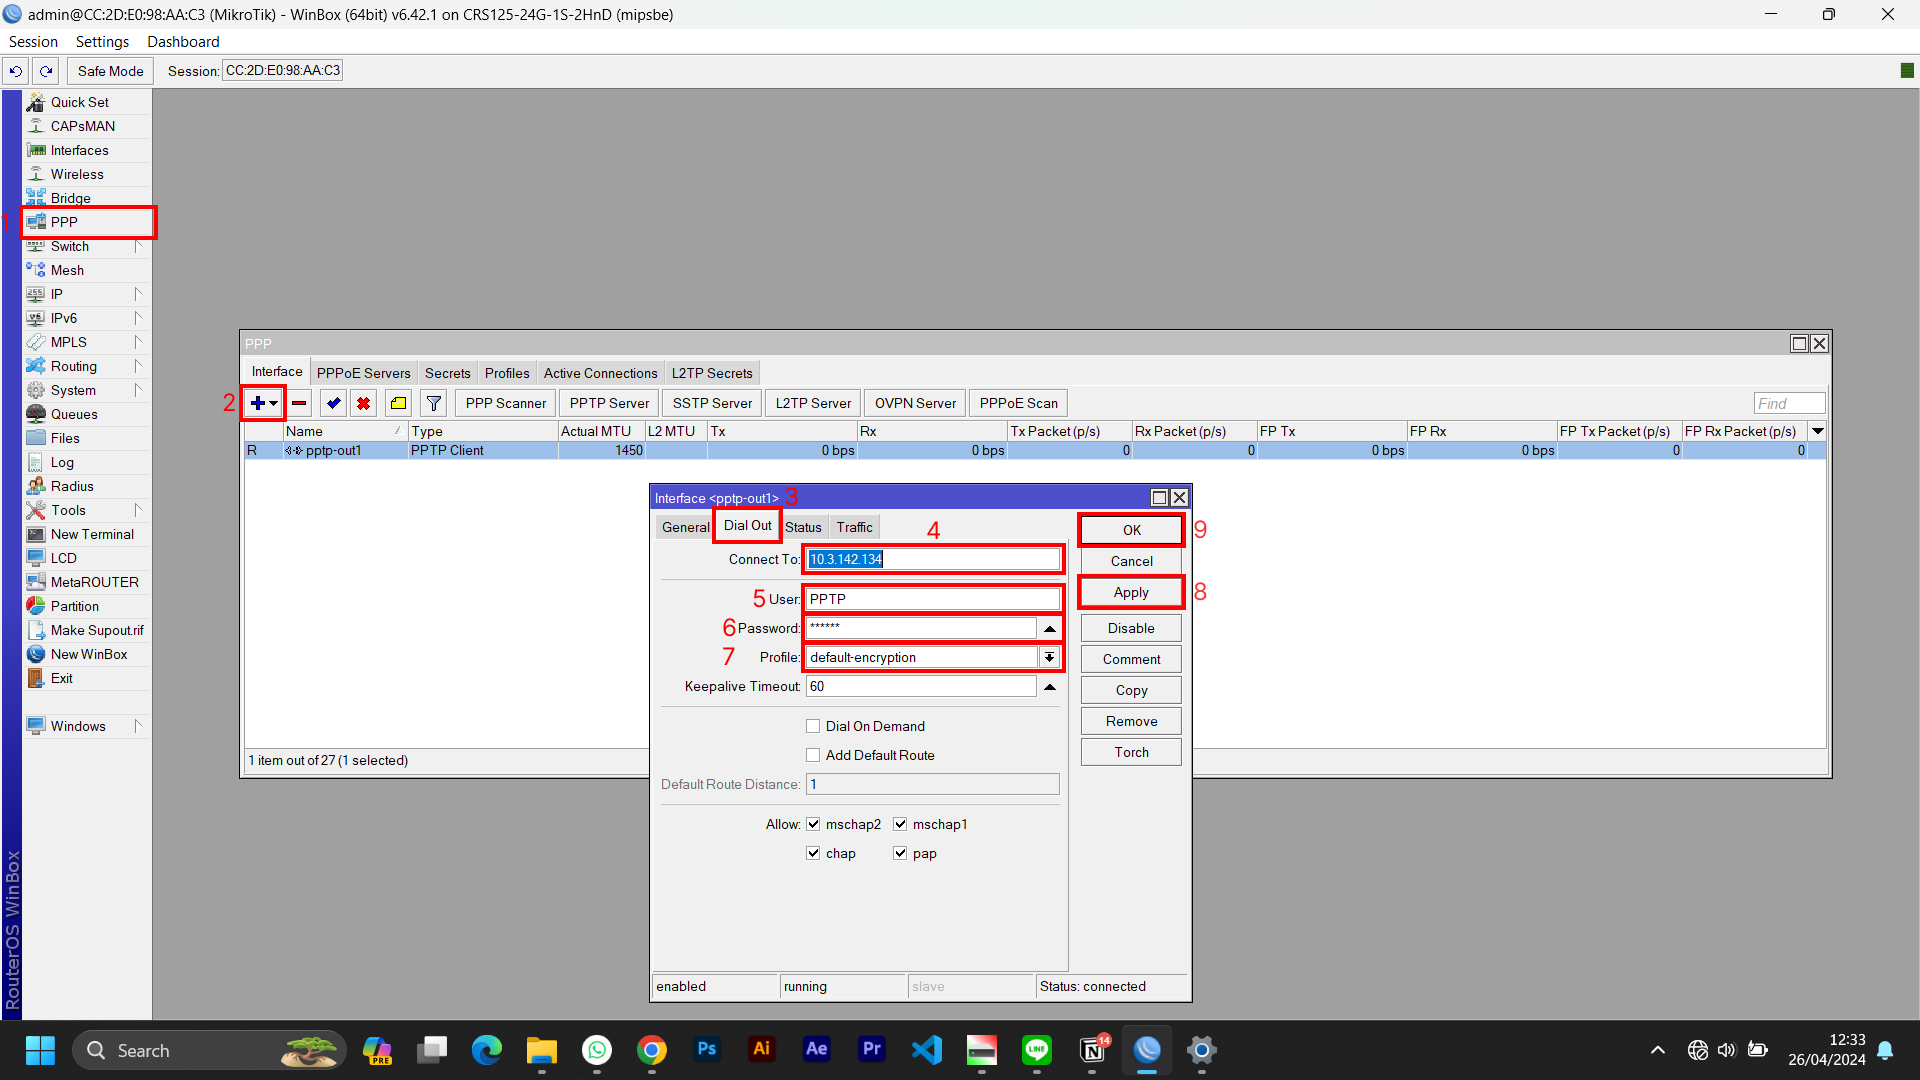
\includegraphics[width=0.8\linewidth]{P4/img/pc2/Step 5.png}
			\caption{Step 5}
			\label{fig:Step 5(PC 2)}
		\end{figure}
    \end{enumerate}

	\textbf{Pengujian Konfigurasi}
	\begin{enumerate}
		\item Lakukan tes ping ke alamat PC1 untuk memastikan VPN PPTP sudah terhubung.
		\begin{figure}[H]
			\centering
			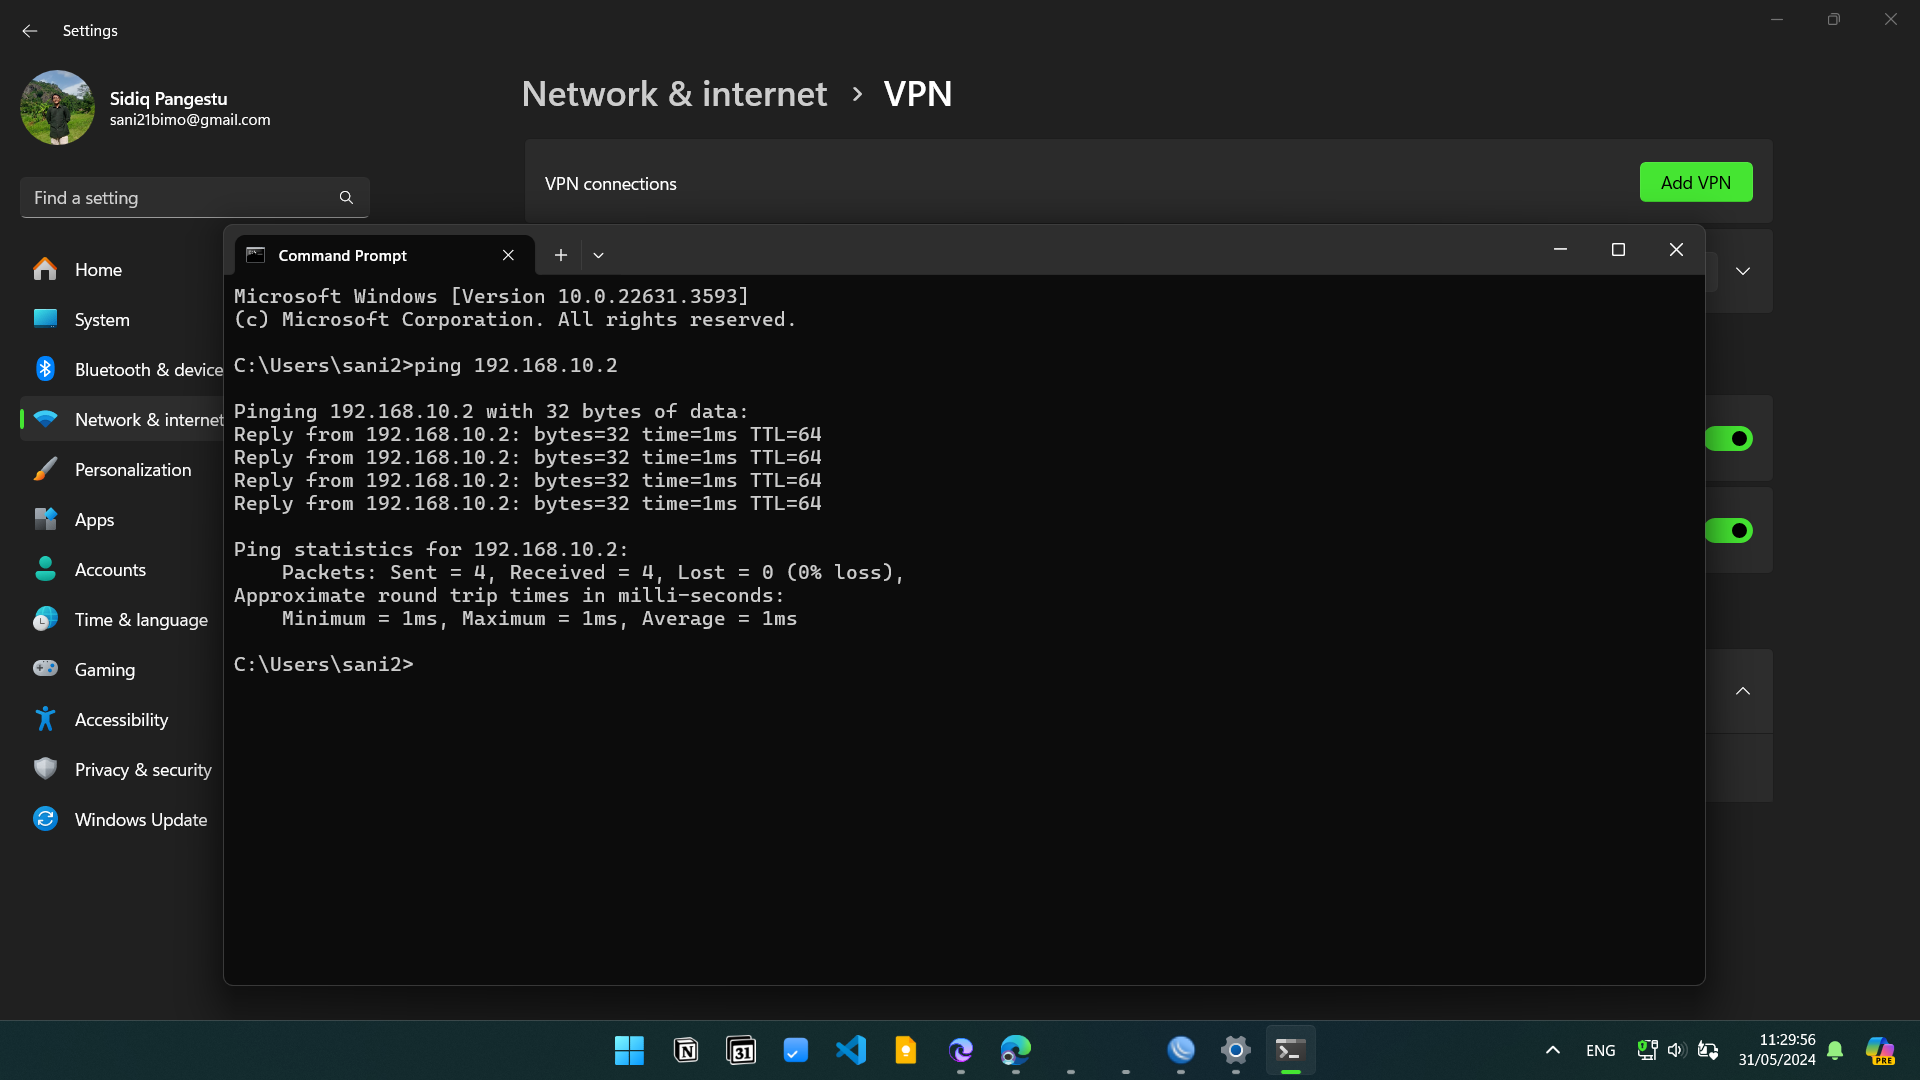
\includegraphics[width=0.8\linewidth]{P4/img/pc2/Step 6.png}
			\caption{Step 1}
			\label{fig:Ping Step 1(PC 2)}
		\end{figure}
	\end{enumerate}
\end{center}

%===========================================================%
\section{Hasil yang didapat}
Memahami penerapan dan penghubungan jaringan dengan menerapkan PPTP dengan VPN

%===========================================================%
\section{Kesimpulan}
Dalam mengkonfigurasi VPN, diperlukan pemahaman dasar mengenai metode PPTP, dan juga diperlukan ketelitian dan fokus agar berhasil

% \section{Tujuan}
\begin{itemize}[label=$\bullet$, itemsep=-1pt, leftmargin=*]
    \item Cek Halo
\end{itemize}

\section{Mengenal Jaringan}
Halo halo

\begin{figure}[H]
    \centering
    \includegraphics[width=0.7\linewidth]{P5/img/contoh.png}
    \caption{Gambar Contoh}
    \label{fig:gambarcontoh}
\end{figure}

\subsection{Tugas Pendahuluan}
\begin{enumerate}
    \item Halo
\end{enumerate}


\begin{center}
    \colorbox{cyan!30}{\parbox{0.8\linewidth}{\textbf{Opsional:} Pelajari Git dan Github. Anda dapat memulai pembelajaran dari sumber berikut ini: \\ \href{https://github.com}{GitHub - https://github.com} \\ \href{https://git-scm.com/doc}{Git -https://git-scm.com/doc}}}
\end{center}


\renewcommand\refname{Daftar Pustaka} % Menghilangkan kata "Daftar Pustaka"
\renewcommand{\bibname}{} % Menghilangkan kata "Bibliography"

\printbibliography
\end{document}